\chapter{多铁材料的设计与理论工具}

\section{多铁材料研究之中的基本方法}

随着对多铁材料研究的进一步深入,越来越多的新的实验、理论方法涌现出来。在实验手段方面,观测设备愈发先进,实验性的电子探针,可以探测电荷的自旋轨道自由度,探测的空间分辨率已经到达元胞尺度,时间分辨率已经达到次飞秒的量级,接近交换作用的时间尺度。激光脉冲沉积也有很大的进展。在理论工具方面,密度泛函理论依然解释多铁性质与预测新的多铁材料的黄金方法\cite{zhong1994phase},在大型系统中第二性原理越来越有价值。基于分子动力学的模拟,如果模型选择合适,其结果完全可以拟合DFT计算的结果。
\begin{figure}[h]
    \centering
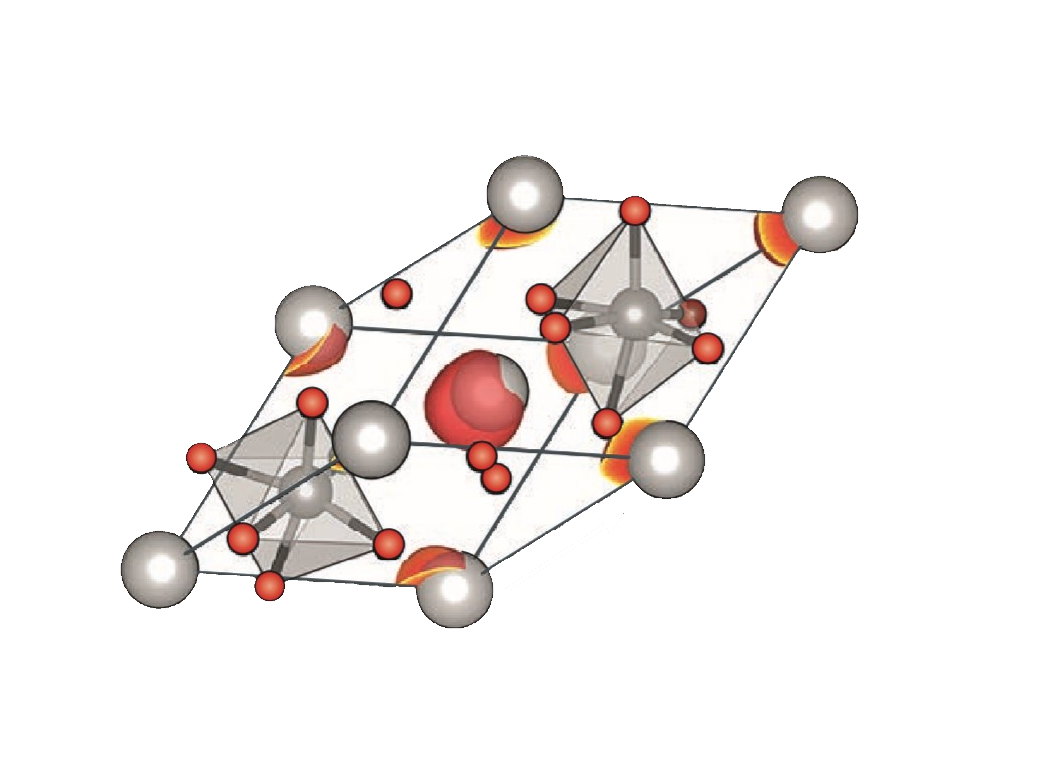
\includegraphics[width=0.8\textwidth]{./pic/007-2.png}
\caption{$BiFeO_{3}$晶体结构}
\label{dog007}
\end{figure}

\section{材料理论设计的基本原理}

结构决定性质,良好的物理性质的背后离不开与之相适应的结构。多年以来的研究成果告诉我们,分子、原子、原子核和电子的运动结构规律的研究离不开量子力学。实验已经证明,量子力学在微观低速领域是正确的,能够对物理现象进行良好的描述以及预测。一般认为,量子力学有着四个基本假定。
\paragraph{第一个假定:}微观粒子的运动状态可以用波函数来描述。
\paragraph{第二个假定:}每个可观测的力学量$\bm{F}$都有一个厄密算符$\bm{\hat{F}} $相对应,力学量的取值只可能是所对应算符的本征值。
\paragraph{第三个假定:}当在一定的运动状态之中测量某力学量$\bm{F}$时,可能得到不同数值,其平均值$\langle \bm{F} \rangle$按照以下公式计算:
\begin{equation}
    \label{eq1}
    \langle F \rangle = \frac{\int \Psi^{*} \hat{F}\Psi d \tau}{\int \Psi^{*} \Psi d \tau}
\end{equation}
\paragraph{第四个假定:}微观粒子的运动方程由薛定谔方程描述
\begin{equation}
    \label{eq2}
    \frac{\partial \Psi}{\partial t}= \frac{i}{\hbar} \hat{H} \Psi
\end{equation}
以上的四个基本假设没有涉及到相对论效应,适用范围为微观低速情况下。

对于宏观物质,尤其是具有$\bm{N_{A}}$量级的原子的物质,这种多粒子系统很难直接应用薛定谔方程直接得到微观粒子的波函数,对于周期性结构的晶体需要采取一些近似手段来大大减少计算量,晶体的空间周期性结构给简化计算工作带来了极大的方便,即使这样,除了少数特殊问题之外严格求解出解析解是不可能的的,通常只能采用数值计算的方法对问题进行理论研究。在进行数值计算时计算的方法可以分为两大类,从头计算和半经验计算。从头计算又叫第一性原理计算,采用真实的物理参数与哈密顿量,从支配客观世界的底层规律入手进行计算。半经验计算则是采用简化版本的哈密顿量,甚至采用基于牛顿力学的某些经验模型,通过实验的结果拟合参数进行计算。

原子中的原子核质量远大于核外电子,所以在研究晶体等周期性结构之中的电子运动时,通常认为原子核的位置是静止不动的,这样系统的波函数可以分解为只包含原子核坐标的$\bm{\Psi_{n}}$和只包含电子坐标的$\bm{\Psi_{e}}$两部分,这就是BO近似,是1927年波恩和奥本海默提出的。

对于单个的球对称原子,可以采用某些数学处理方法进行简化为径向方程求解,但对于多体问题,尤其时不存在球对称性的多体问题需要采取别的方法。量子力学的线性组合原理提供了一个良好的思路。电子的轨道波函数$\phi_{i}$可以表示为一系列的基函数$\eta_{j}$的线性组合。
\begin{equation}
    \label{eq3}
    \phi_{i} = \sum_{j} c_{ij} \eta_{j}
\end{equation}
其中$c_{ij}$为组合系数。如果系统内的任意波函数都可以表示为一组基函数的线性组合,这一组基函数可以称为完备的基组。在实际应用时,自然不可能将波函数展开到所有的基函数,只能选取有限多个基函数的组合来趋近于真实的波函数。如果将电子的波函数展开成有限个基函数的线性组合,对波函数的变分也就转化成为对若干系数的变分,这使得数值计算变得更加可能。

这些基函数的选取方式由很多种,在具有周期性结构的晶体或者有周期性边界条件时可以选取平面波作为基函数,在研究分子问题时可以采用原子轨道作为基函数。随着数值计算方法的发展,为了适应不同研究条件不同研究层次不同研究对象,人们提出了很多基函数。斯莱特型轨道(STO)是一种常用的基函数,基于对氢原子轨道的模仿,有着极强的物理意义。
\begin{equation}
    \label{sto}
    \eta^{STO}=Nr^{n-1}exp(-\zeta r)Y_{l,m}(\theta,\phi)
\end{equation}
其中N为归一化常数,$Y_{l,m}(\theta,\phi)$为球谐函数。高斯型轨道(GTO)也是一种比较常见的基函数
\begin{equation}
    \label{gto}
    \eta^{GTO}=Nx^{i}y^{j}z^{k}exp(-\alpha r^{2})
\end{equation}
其中$\alpha$时轨道指数$L=i+j+k$与轨道的具体形式有关L=0,1,2分别对应s,p,d轨道。对于周期性边界条件,平面波是一种好合适的基函数组,但平面波也有局限性,其收敛慢,计算时间长占用资源多,对数值计算十分不利,通过对平面波与原子轨道相结合,在靠近原子核附近时采用原子轨道,在远离原子核的地方采用平面波形成的缀加平面波(PWA)也是一种常见的基函数组。

从上面这些近似看来,即使是第一性原理计算,也不可避免的引入很多近似,如波恩-奥本海默近似、采用非相对论量子力学忽略了相对论效应、采用有限多个基函数组合等,计算结果与实际仍会有偏离,在某些特殊情况下会产生较大的偏差,针对不同的情况条件与研究对象,需要采取不同的手段对计算过程进行修正,以防产生系统性的错误。

\subsection{晶体场理论与配位场理论}
在研究凝聚态物质之中,价键理论也是一种重要的研究手段,虽然能带论仍然是主要的研究方法与手段,但价键理论作为一种成熟的化学理论也有其独特的理论与应用价值。在研究晶格畸变,几何构型等问题时,价键理论,特别时晶体场理论,有着重要的作用。

\begin{figure}[h]
    \centering
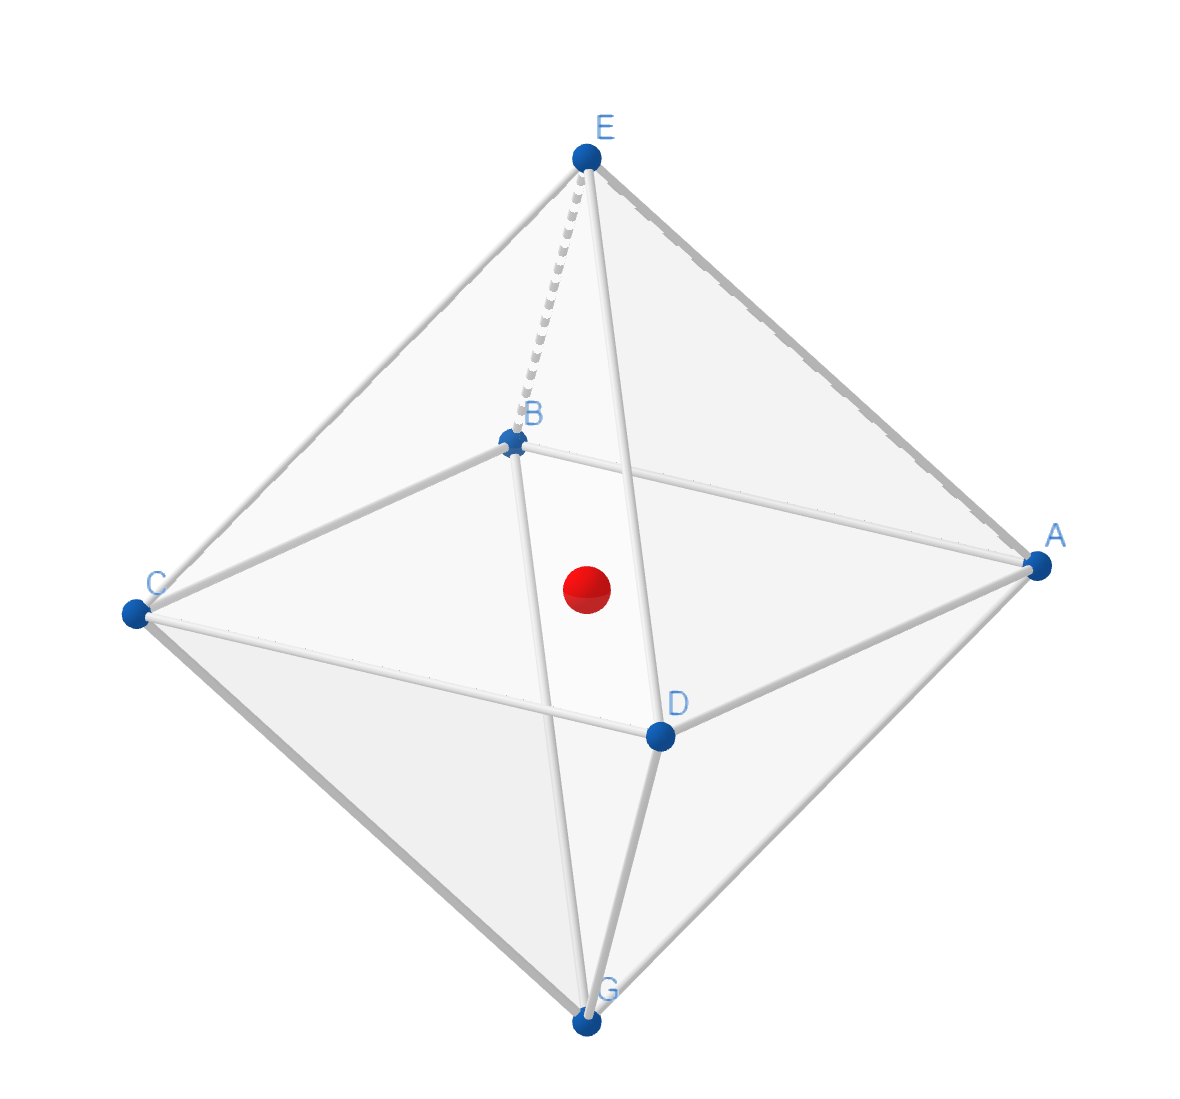
\includegraphics[width=0.8\textwidth]{./pic/p001.png}
\caption{Ti原子在氧八面体的正中心}

\label{dogp01}
\end{figure}
在氢原子的情况下,没有其他的外加条件的情况下,波函数中的主量子数n有着$n^{2}$度简并
,在更复杂的条件下,量子系统中的简并度会受到外加条件的影响而进一步减小。在周期性结构的晶格格点之上,受到周围各向异性排布的其他原子或离子的影响,原子或离子的能级会发生变化。晶体场理论主要是研究在各向异性环境中的原子,根具晶场效应的强弱,可以分为三类。

\paragraph{弱晶场(交换劈裂>自旋轨道耦合>晶场)}
稀土元素是一个典型的例子,稀土元素的4f电子距离原子核比较近,不容易受到其他离子势场的影响,这种情况下弱晶场对系统的影响不大,排在自旋轨道耦合之后。
\paragraph{中晶场(交换劈裂>晶场>自旋轨道耦合)}
过度金属,尤其是3d金属是一个典型的例子,晶场效应大于自旋轨道耦合,洪特定则部分失效,导致轨道磁矩猝灭。
\paragraph{强晶场(晶场>交换劈裂>自旋轨道耦合)}
在这种情况下晶场效应足够强大,以至于洪特定则完全失效,不同层级的波函数可以发生混合,通常发生在4d或5d化合物中间,同时要考虑到中心阳离子的d轨道可能会同外围阴离子的p轨道发生混合,形成部分共价键。这种情况常常是配位场理论的研究范围。

\subsubsection{过渡金属离子的晶体场效应}
对于中等程度的晶体场,过度金属是一个很好的例子。典型的钙钛矿结构的$\text{LaTiO}_{3}$中的$Ti^{3+}$离子。在$\text{LaTiO}_{3}$中$La^{3+}\text{和}O^{2-}$没有未配对电子。系统的磁矩主要是由$Ti^{3+}$的单个未配对电子决定的。这个带有磁矩的未配对电子不仅受到中心阳离子的经典库伦吸引力的影响,而且受到到组成周围氧八面体的六个阴离子的影响,其哈密顿量为:
\begin{equation}
    \mathcal{H}_{3d}(\bm{r})=\mathcal{H}^{\text{(Ti)}}(\bm{r})+\sum^{6}_{\text{j=1}}V^{\text{(O)}}(\bm{r}-\bm{R}_{j})
\end{equation}
除了直接求解薛定谔方程,还可以通过3d轨道的分布规律和氧八面体的几何对称性定性地得到。自由粒子的3d轨道是五重简并的,可以细分为$d_{x^{2}-y^{2}},d_{z^{2}},d_{xy},d_{yz}\text{和}d_{zx}$。在氧八面体内部,前两种d轨道$d_{x^{2}-y^{2}},d_{z^{2}}$的波函数主瓣指向带有负电的氧离子,能级会提高,后三种d轨道$d_{xy},d_{yz}\text{和}d_{zx}$波函数的主瓣方向指向氧八面体中的氧正方形的对角线方向,没有正对着氧离子。能级会下降。五重简并就这样被解除了,分为两组,一组是能量较高的二重态$e_{g}$,和剩下的一组能量降低的三重态$t_{2g}$。与$\text{LaTiO}_{3}$相类似的$La_{2}CuO_{4}$中的$Cu^{2+}$也是由氧八面体包围,也带有一个未成对电子,不同的是对于$Cu^{2+}$d轨道存在9个电子,对应应该考虑空穴的占据状态。

% \begin{figure}[h]
%     \centering
%     \resizebox{\textwidth}{!}{
%     \begin{tikzpicture}[line cap=round,line join=round,>=triangle 45,x=0.4cm,y=0.4cm]
%         \clip(-7.568420055431509,-14.648982459713856) rectangle (30.651216037856322,15.468248877500034);
%         \draw [line width=2pt] (-5,0)-- (5,0);
%         \draw [line width=2pt] (0,5)-- (0,-5);
%         \draw [rotate around={-50.05724853255913:(-0.585,0.685)},line width=2pt,color=uququq,fill=uququq,fill opacity=0.53] (-0.585,0.685) ellipse (0.9009667929793787 and 0.4102330582139209);
%         \draw [rotate around={-129.94275146744084:(0.585,0.685)},line width=2pt,color=uququq,fill=uququq,fill opacity=0.66] (0.585,0.685) ellipse (0.9009667929793787 and 0.4102330582139209);
%         \draw [rotate around={50.05724853255913:(-0.585,-0.685)},line width=2pt,color=uququq,fill=uququq,fill opacity=0.72] (-0.585,-0.685) ellipse (0.9009667929793787 and 0.4102330582139209);
%         \draw [rotate around={129.94275146744087:(0.585,-0.685)},line width=2pt,color=uququq,fill=uququq,fill opacity=0.69] (0.585,-0.685) ellipse (0.9009667929793787 and 0.4102330582139209);
%         \draw (2.114941726218458,4.520121475389473) node[anchor=north west] {$\mathbf{d_{xy},d_{yz},d_{zx}}$};
%         \draw [line width=2pt] (7,0)-- (17,0);
%         \draw [line width=2pt] (12,5)-- (12,-5);
%         \draw [line width=2pt] (19,0)-- (29,0);
%         \draw [line width=2pt] (24,5)-- (24,-5);
%         \draw [rotate around={90:(12,1.1638436934424887)},line width=2pt,fill=black,fill opacity=0.39] (12,1.1638436934424887) ellipse (1.2260171011811196 and 0.38546827317293436);
%         \draw [rotate around={180:(10.83615630655751,0)},line width=2pt,fill=black,fill opacity=0.2] (10.83615630655751,0) ellipse (1.2260171011811196 and 0.38546827317293436);
%         \draw [rotate around={-90:(12,-1.1638436934424887)},line width=2pt,fill=black,fill opacity=0.2] (12,-1.1638436934424887) ellipse (1.2260171011811196 and 0.38546827317293436);
%         \draw [rotate around={0:(13.16384369344249,0)},line width=2pt,fill=black,fill opacity=0.2] (13.16384369344249,0) ellipse (1.2260171011811196 and 0.38546827317293436);
%         \draw [rotate around={0:(24.00254899481813,0)},line width=2pt,fill=black,fill opacity=0.2] (24.00254899481813,0) ellipse (1.6839389847634159 and 0.7648916185947887);
%         \draw [rotate around={90:(24,1.4398026937089552)},line width=2pt,fill=black,fill opacity=0.2] (24,1.4398026937089552) ellipse (1.4398026937087463 and 0.7020750078174347);
%         \draw [rotate around={-90:(24,-1.4398026937089552)},line width=2pt,fill=black,fill opacity=0.2] (24,-1.4398026937089552) ellipse (1.4398026937087463 and 0.7020750078174347);
%         \draw (14.130215120592297,4.520121475389473) node[anchor=north west] {$\mathbf{d_{x^{2}-y^{2}}}$};
%         \draw (26.105964589326746,4.520121475389473) node[anchor=north west] {$\mathbf{d_{z^{2}}}$};
%         \begin{scriptsize}
%         \draw [fill=ududff] (-5,0) circle (2.5pt);
%         \draw [fill=ududff] (5,0) circle (2.5pt);
%         \draw [fill=ududff] (0,5) circle (2.5pt);
%         \draw [fill=ududff] (0,-5) circle (2.5pt);
%         \draw [fill=ududff] (7,0) circle (2.5pt);
%         \draw [fill=ududff] (17,0) circle (2.5pt);
%         \draw [fill=ududff] (12,5) circle (2.5pt);
%         \draw [fill=ududff] (12,-5) circle (2.5pt);
%         \draw [fill=xdxdff] (19,0) circle (2.5pt);
%         \draw [fill=xdxdff] (29,0) circle (2.5pt);
%         \draw [fill=ududff] (24,5) circle (2.5pt);
%         \draw [fill=ududff] (24,-5) circle (2.5pt);
%         \draw [fill=uuuuuu] (12,0) circle (2pt);
%         \end{scriptsize}
%         \end{tikzpicture}
%     }
%     \vspace*{-3cm}
%     \caption{氧八面体中心离子的d轨道\ 简并的5个d轨道由于处于各向异性的势场中,地位不再等同,发生能级分裂,波函数主瓣指向阴离子的轨道能量会上升,波函数主瓣远离阴离子,指向其空隙的能级会下降。}
%     \label{t001}
% \end{figure}


\definecolor{uuuuuu}{rgb}{0.26666666666666666,0.26666666666666666,0.26666666666666666}
\definecolor{xdxdff}{rgb}{0.49019607843137253,0.49019607843137253,1}
\definecolor{uququq}{rgb}{0.25098039215686274,0.25098039215686274,0.25098039215686274}
\definecolor{ududff}{rgb}{0.30196078431372547,0.30196078431372547,1}

\begin{figure}[h]
    \centering
    \resizebox{\textwidth}{!}{
    \vspace*{-3cm}
    \begin{tikzpicture}[line cap=round,line join=round,>=triangle 45,x=0.4cm,y=0.4cm]
        \clip(-7.568420055431509,-14.648982459713856) rectangle (30.651216037856322,15.468248877500034);
        \draw [line width=2pt] (-5,0)-- (5,0);
        \draw [line width=2pt] (0,5)-- (0,-5);
        \draw [rotate around={-50.05724853255913:(-0.585,0.685)},line width=2pt,color=uququq,fill=uququq,fill opacity=0.53] (-0.585,0.685) ellipse (0.9009667929793787 and 0.4102330582139209);
        \draw [rotate around={-129.94275146744084:(0.585,0.685)},line width=2pt,color=uququq,fill=uququq,fill opacity=0.66] (0.585,0.685) ellipse (0.9009667929793787 and 0.4102330582139209);
        \draw [rotate around={50.05724853255913:(-0.585,-0.685)},line width=2pt,color=uququq,fill=uququq,fill opacity=0.72] (-0.585,-0.685) ellipse (0.9009667929793787 and 0.4102330582139209);
        \draw [rotate around={129.94275146744087:(0.585,-0.685)},line width=2pt,color=uququq,fill=uququq,fill opacity=0.69] (0.585,-0.685) ellipse (0.9009667929793787 and 0.4102330582139209);
        \draw (2.114941726218458,4.520121475389473) node[anchor=north west] {$\mathbf{d_{xy},d_{yz},d_{zx}}$};
        \draw [line width=2pt] (7,0)-- (17,0);
        \draw [line width=2pt] (12,5)-- (12,-5);
        \draw [line width=2pt] (19,0)-- (29,0);
        \draw [line width=2pt] (24,5)-- (24,-5);
        \draw [rotate around={90:(12,1.1638436934424887)},line width=2pt,fill=black,fill opacity=0.39] (12,1.1638436934424887) ellipse (1.2260171011811196 and 0.38546827317293436);
        \draw [rotate around={180:(10.83615630655751,0)},line width=2pt,fill=black,fill opacity=0.2] (10.83615630655751,0) ellipse (1.2260171011811196 and 0.38546827317293436);
        \draw [rotate around={-90:(12,-1.1638436934424887)},line width=2pt,fill=black,fill opacity=0.2] (12,-1.1638436934424887) ellipse (1.2260171011811196 and 0.38546827317293436);
        \draw [rotate around={0:(13.16384369344249,0)},line width=2pt,fill=black,fill opacity=0.2] (13.16384369344249,0) ellipse (1.2260171011811196 and 0.38546827317293436);
        \draw [rotate around={0:(24.00254899481813,0)},line width=2pt,fill=black,fill opacity=0.2] (24.00254899481813,0) ellipse (1.6839389847634159 and 0.7648916185947887);
        \draw [rotate around={90:(24,1.4398026937089552)},line width=2pt,fill=black,fill opacity=0.2] (24,1.4398026937089552) ellipse (1.4398026937087463 and 0.7020750078174347);
        \draw [rotate around={-90:(24,-1.4398026937089552)},line width=2pt,fill=black,fill opacity=0.2] (24,-1.4398026937089552) ellipse (1.4398026937087463 and 0.7020750078174347);
        \draw (14.130215120592297,4.520121475389473) node[anchor=north west] {$\mathbf{d_{x^{2}-y^{2}}}$};
        \draw (26.105964589326746,4.520121475389473) node[anchor=north west] {$\mathbf{d_{z^{2}}}$};
        \begin{scriptsize}
        \draw [fill=ududff] (-5,0) circle (2.5pt);
        \draw [fill=ududff] (5,0) circle (2.5pt);
        \draw [fill=ududff] (0,5) circle (2.5pt);
        \draw [fill=ududff] (0,-5) circle (2.5pt);
        \draw [fill=ududff] (7,0) circle (2.5pt);
        \draw [fill=ududff] (17,0) circle (2.5pt);
        \draw [fill=ududff] (12,5) circle (2.5pt);
        \draw [fill=ududff] (12,-5) circle (2.5pt);
        \draw [fill=xdxdff] (19,0) circle (2.5pt);
        \draw [fill=xdxdff] (29,0) circle (2.5pt);
        \draw [fill=ududff] (24,5) circle (2.5pt);
        \draw [fill=ududff] (24,-5) circle (2.5pt);
        \draw [fill=uuuuuu] (12,0) circle (2pt);
        \end{scriptsize}
        \end{tikzpicture}
    }
    \vspace*{-3cm}
    \caption{氧八面体中心离子的d轨道\ 简并的5个d轨道由于处于各向异性的势场中,地位不再等同,发生能级分裂,波函数主瓣指向阴离子的轨道能量会上升,波函数主瓣远离阴离子,指向其空隙的能级会下降。}
    \label{}
\end{figure}

\begin{figure}[h]
    \centering
    \resizebox{\textwidth}{!}{
        \vspace*{-3cm}
        \begin{tikzpicture}[line cap=round,line join=round,>=triangle 45,x=3cm,y=3cm]
            \clip(-4.880291166623681,-2.3485074264249626) rectangle (5.396326222588918,6.000589473883519);
            \draw [->,line width=2pt] (-1,2) -- (1,2);
            \draw [->,line width=2pt] (1,1.5) -- (-1,1.5);
            \draw (-0.31386821851793875,1.4436796223977102) node[anchor=north west] {\parbox{3.167610477296026 cm}{\Huge 温度 \\ 压强 \\ 光照}};
            \draw [line width=2pt] (-2.5,2.5)-- (-2,2.5);
            \draw [line width=2pt] (-3.5,2.5)-- (-3,2.5);
            \draw [line width=2pt] (3.5,2.5)-- (3,2.5);
            \draw [line width=2pt] (2.5,2.5)-- (2,2.5);
            \draw [line width=2pt] (-2.5,1)-- (-3,1);
            \draw [line width=2pt] (-2,1)-- (-1.5,1);
            \draw [line width=2pt] (-3.5,1)-- (-4,1);
            \draw [line width=2pt] (2.5,1)-- (3,1);
            \draw [line width=2pt] (2,1)-- (1.5,1);
            \draw [line width=2pt] (3.5,1)-- (4,1);
            \draw [->,line width=2pt] (-3.9,0.8) -- (-3.9,1.2);
            \draw [->,line width=2pt] (-3.6,1.2) -- (-3.6,0.8);
            \draw [->,line width=2pt] (-2.9,0.8) -- (-2.9,1.2);
            \draw [->,line width=2pt] (-2.6,1.2) -- (-2.6,0.8);
            \draw [->,line width=2pt] (-1.9,0.8) -- (-1.9,1.2);
            \draw [->,line width=2pt] (-1.6,1.2) -- (-1.6,0.8);
            \draw [->,line width=2pt] (1.6,0.8) -- (1.6,1.2);
            \draw [->,line width=2pt] (1.9,1.2) -- (1.9,0.8);
            \draw [->,line width=2pt] (2.7,0.8) -- (2.7,1.2);
            \draw [->,line width=2pt] (3.7,0.8) -- (3.7,1.2);
            \draw [->,line width=2pt] (2.2,2.3) -- (2.2,2.7);
            \draw [->,line width=2pt] (3.2,2.3) -- (3.2,2.7);
            \draw (-3.0680028808603987,0.5637246165935542) node[anchor=north west] {\parbox{5 cm}{\Huge 低自旋态 \\ S=0}};
            \draw (2.4107645957534545,0.5532489617625523) node[anchor=north west] {\parbox{5 cm}{\Huge 高自旋态 \\ S=2}};
            \end{tikzpicture}
    }
    \vspace*{-3cm}
    \caption{在八面体络合物中$Fe^{2+}$能级示意图,在一定条件下两种自旋状态可以相互转化}
    \label{t002}
\end{figure}

\subsubsection{JT效应}
Jahn-Teller定理指出,在对称的非线性分子之中,如果一个体系存在多个简并能级,就会发生自发畸变使得简并消除。仍然以$\text{LaTiO}_{3}$为例子,$Ti^{3+}$处于氧八面体的中心位置,在正常情况下$Ti^{3+}$的五个3d轨道是简并的。在进入氧八面体的形成的各向异性的势场之后,会发生能级分裂,分成两组,三重态$t_{2g}$与二重态$e_{g}$。能量简并情况仍然存在,如果氧八面体沿着z轴方向发生一个拉长$\delta_{z}$,这样z轴方向上的离子距离会变得和xy轴不一样,这样会使得能级发生进一步分裂。

\begin{figure}[h]
    \centering
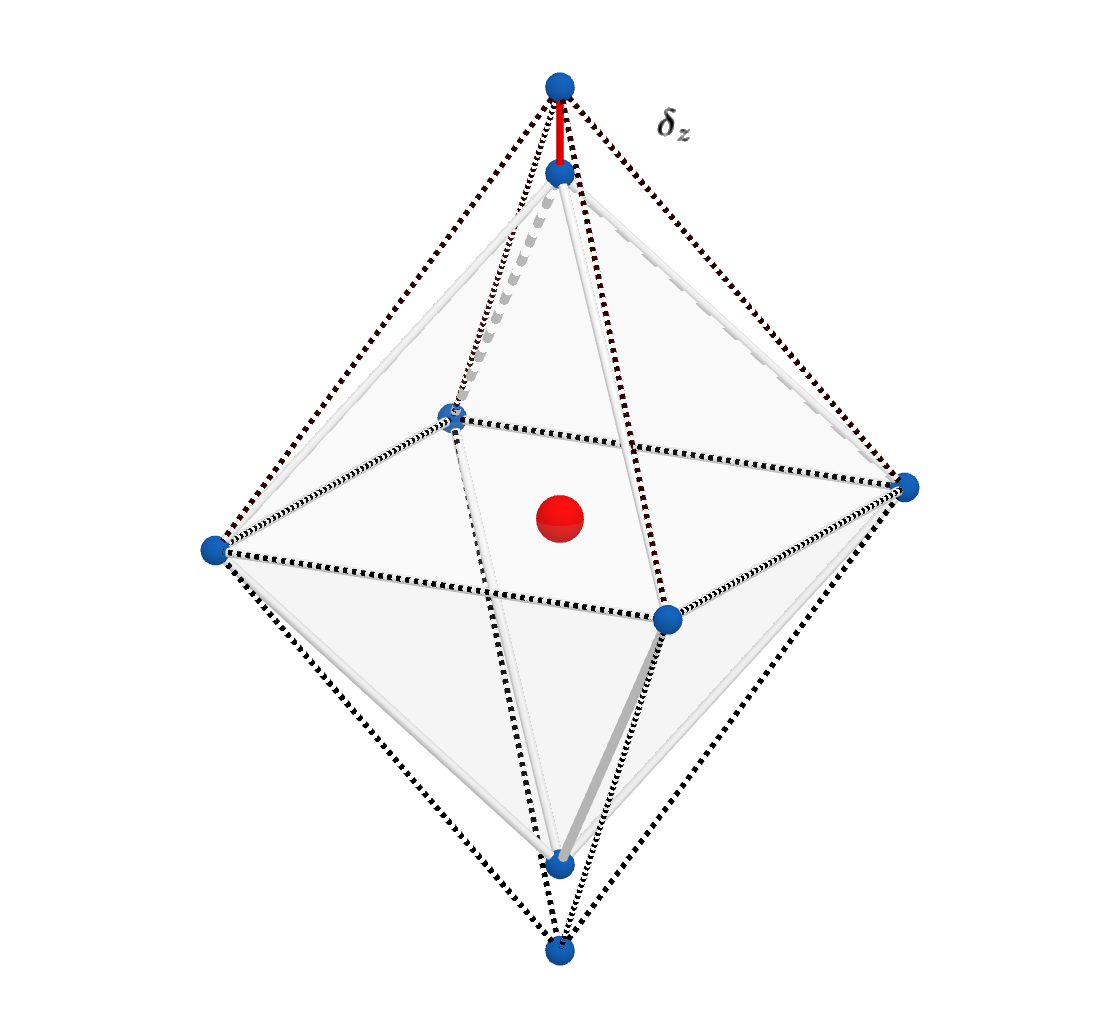
\includegraphics[width=0.8\textwidth]{./pic/p002.png}
\caption{JT效应使得氧八面体发生畸变}

\label{dogp02}
\end{figure}

在$\text{LaTiO}_{3}$发生畸变的情况下,弹性形变使得能量升高$\alpha \delta_{z}^{2}$,电子能级的改变造成的总能量变化与形变值成正比,能量变化为$-\beta \delta_{z}$
。发生形变所造成的整个能量变化为$\alpha \delta_{z}^{2} -\beta \delta_{z}$,这是一个典型的二次函数关系。当能量增量取最小值时$\delta_{z}=\beta /2\alpha $,当整个体系的能量降低时,Jahn-Teller效应就会自发发生。

Jahn-Teller效应最早是在研究分子现象时被发现的,随后推广到晶体之中,在晶体中的Jahn-Teller效应相当复杂。不同的分子或晶格结构会发生不同形式的形变,轨道有序化也伴随着Jahn-Teller配合体有序化,但有些情况下Jahn-Teller效应并不与轨道有序化相耦合,在另一些情况下,Jahn-Teller效应也可能与磁有序相耦合,总之,这是一种相当复杂的效应。

\subsubsection{配位场理论}

在强晶体场的情况下,周围各向异性的离子产生的势能对中心原子或离子的能级影响如此之大以至于可以通过配位的方式形成配位键,这种情况通常出现在过渡金属化合物或配合物,配位基一般是非金属的原子或者分子,常见的主要有$TiF_{6}^{3-}\text{,}Fe(CN)_{6}^{4-}$。通常在处理配位场问题时,需要按照共价键的通用研究方法,考虑共价键、分子轨道等来进行综合考虑。

配位场中的能量分裂也会影响中心离子的磁学性质。以$[Cr(H_{2}O)_{2}]^{2+}$为例,Cr在水分子八面体的各向异性势场当中会发生能级分裂,会分为三重态能量较低的$t_{2g}$和能量比较高的二重态$e_{g}$。Cr有四个价电子,能级较低的$t_{2g}$只能填入三个自旋相同的电子,剩下的那一个电子有两种填充方式,一种时以自旋反平行填充在能级比较低的$t_{2g}$,这种方式所有价电子自旋方向不完全相同,称为低自旋态,另一种是以自旋平行的状态填充到能级较高的$e_{g}$,这种方式所有价电子自旋方向相同,称为高自旋态。具体这两种填充方法在真实情况下如何选择,归根结底还是要整体考虑,看哪一种填充方式总能量更低。通常来讲,周围配位场所造成的能级分裂大小$\Delta$是低自旋态与高自旋态的决定性因素,大的$\Delta$值有利于低自旋态,$\cancel{\Delta}$小则有助于低自旋态的产生。从经验上看来,在d层价电子大于等于八个或者小于等于三个的情况下,有着比较明确的情况,配合物一定会处于高自旋态,但在其他情况下,高自旋态与低自旋态两种情况都有可能出现。在0K的理想条件下,这取决与能量的大小,但在更复杂一些的情况下,多样的外在条件会导致高自旋态与低自旋态之间的转换。例如在八面体中间变得$Fe^{2+}$,其低自旋态的能量稍小于高自旋态的能量,在接近0k的低温下为低自旋态,当温度达到一定程度时,会从低自旋态自发向高自旋态转化,在温度比较高的时候,高自旋态的熵$\Delta S$的影响超过能量的影响,高自旋态的热力学稳定性会提高。


\begin{table}[!htbp]
    \caption{八面体配合物的高自旋态与低自旋态}
    \label{tab:bmt}
    \resizebox{\textwidth}{!}{
    \begin{tabular}{c|c|c|c|c|c|c|c|c}
        \toprule
        \multirow{2}*{$n_{d}$(d电子数)}&\multicolumn{4}{|c|}{高自旋态}&\multicolumn{4}{|c}{低自旋态}\\
        \cline{2-9}
        &$t_{2g}$&$e_{g}$&n&p&$t_{2g}$&$e_{g}$&n&p\\
        \hline
        1&\sout{↑\ }\ \sout{\ \ }\ \sout{\ \ }&\sout{\ \ }\ \sout{\ \ }&1&1.73&&&&\\
        \hline
        2&\sout{↑\ }\ \sout{↑\ }\ \sout{\ \ }&\sout{\ \ }\ \sout{\ \ }&2&2.83&&&&\\
        \hline
        3&\sout{↑\ }\ \sout{↑\ }\ \sout{↑\ }&\sout{\ \ }\ \sout{\ \ }&3&3.87&&&&\\
        \hline
        4&\sout{↑\ }\ \sout{↑\ }\ \sout{↑\ }&\sout{↑\ }\ \sout{\ \ }&4&4.90&\sout{↑↓}\ \sout{↑\ }\ \sout{↑\ }&\sout{\ \ }\ \sout{\ \ }&2&2.83\\
        \hline
        5&\sout{↑\ }\ \sout{↑\ }\ \sout{↑\ }&\sout{↑\ }\ \sout{↑\ }&5&5.92&\sout{↑↓}\ \sout{↑↓}\ \sout{↑\ }&\sout{\ \ }\ \sout{\ \ }&1&1.73\\
        \hline
        6&\sout{↑↓}\ \sout{↑\ }\ \sout{↑\ }&\sout{↑\ }\ \sout{↑\ }&4&4.90&\sout{↑↓}\ \sout{↑↓}\ \sout{↑↓}&\sout{\ \ }\ \sout{\ \ }&0&0\\
        \hline
        7&\sout{↑↓}\ \sout{↑↓}\ \sout{↑\ }&\sout{↑\ }\ \sout{↑\ }&3&3.87&\sout{↑↓}\ \sout{↑↓}\ \sout{↑↓}&\sout{↑\ }\ \sout{\ \ }&1&1.73\\
        \hline
        8&\sout{↑↓}\ \sout{↑↓}\ \sout{↑↓}&\sout{↑\ }\ \sout{↑\ }&2&2.83&&&&\\
        \hline
        9&\sout{↑↓}\ \sout{↑↓}\ \sout{↑↓}&\sout{↑↓}\ \sout{↑\ }&1&1.73&&&&\\
        \bottomrule
    \end{tabular}
    }
\end{table}


\subsection{海森堡模型}

假设在晶体的周期性结构中的格点上面有两个自旋未配对的d电子。根据量子力学以及泡利不相容原理,两个d电子之间的交换能:
\begin{equation}
    E_{ex}=\pm \bm{J}_{12}=\pm \int \phi_{1}^{*}(\bm{r}_{1})\phi_{2}^{*}(\bm{r}_{2})V(\bm{r}_{12})\phi_{1}(\bm{r}_{2})\phi_{2}(\bm{r}_{1})d\bm{r}_{1}d\bm{r}_{2}
    \label{eq:hsb1}
\end{equation}
其中$V(\bm{r})$为系统的库伦相互作用势能,公式中符号对应着自旋的方向。+对应着两个电子自旋方向相反,-号对应两个电子自旋方向相同。

如果考虑到每个离子晶格上未成对的电子大于一个,即每个格点上带有是自旋大于$\frac{1}{2}$,同时忽略同一个离子格点上不同电子之间的交换作用,同时认为量格点上所有电子的交换积分相同,可以得到:
\begin{equation}
    H = -\sum_{l,l'} J_{ll'}\hat{\bm{S}}_{l}\cdot\hat{\bm{S}}_{l'} \ \text{,}\ (l \neq l' )
    \label{eq:hsb2}
\end{equation}
其中$\hat{\bm{S}}_{l}$为在l格点上的自旋算符,$\hat{\bm{S}}_{l‘}$为在l’格点上的自旋算符,$\bm{J}_{ll'}$是格点上电子间的交换积分:
\begin{equation}
    \bm{J}_{ll'}=\bm{J}(|\bm{l}-\bm{l'}|)
    \label{eq:hsb3}
\end{equation}
公式(\ref{eq:hsb2})就是著名的海森堡模型。在实际应用的时候,考虑到交换作用是一种近距离的作用,在长程作用上对整个系统的影响可以忽略不计,在对一般问题的研究中可以只考虑近距离的,尤其是只考虑最近邻的电子交换作用,在各项同性的情况下,海森堡模型可以进一步化简:
\begin{equation}
    H=-J\sum_{l,\delta}\hat{\bm{S}}_{l}\cdot \hat{\bm{S}}_{l+\delta}
    \label{eq:hsb4}
\end{equation}
其中$\delta$为两格点之间的正格矢。当J>0时$\hat{\bm{S}}_{1}\cdot\hat{\bm{S}}_{2}$为正时能量最低,两其个电子自旋方向平行,基态通常为铁磁性。相反的,当J<0时$\hat{\bm{S}}_{1}\cdot\hat{\bm{S}}_{2}$为负时能量最低,两其个电子自旋方向反平行,基态通常为反铁磁性。

海森堡模型的相互作用哈密顿量在时间反演的情况下是不变的,在时间反演操作下,由运动电流产生的磁矩会反向,相互作用哈密顿量会由于两次反向而保持不变,但在外加磁场的情况下,系统的哈密顿量会多出一种外加磁场项$\bm{H}\cdot\bm{S}$这一项会发生改变,外加磁场会破坏系统的时间反演对称性。

\subsection{能带论计算方法}
基于单电子近似能带理论是凝聚态物理的核心问题,多粒子系统中的电子性质的一个有效的解决方法。基于单电子近似的近自由电子理论与紧束缚模型固然可以给出多粒子体系大周期性结构物质之中电子运动的清晰的物理图像,但与实验结果相比偏差过大,难以达到实际使用的要求与应用标准。需要采用更加精确更加可靠的计算方法,如正交平面波方法、赝势法、追加平面波法。这些方法的区别主要在于展开波函数的函数集不同以及用来代替真实晶格之中周期性势能的有效势选取不同。

\subsubsection{正交平面波法}

在周期性结构之中,傅里叶变换是最常用的分析方法之一,傅里叶分解产生的平面波是最简单的正交完备函数集之一。
\begin{equation}
    |\bm{k}+\bm{G}\rangle =\Omega^{-\frac{1}{2}} e^{i(\bm{k}+\bm{G})\cdot\bm{r}}
\end{equation}
晶体之中的波函数可以用平面波展开:
\begin{equation}
    \psi_{\bm{k}(\bm{r})}=\Omega^{-\frac{1}{2}}\sum_{\bm{G}}c(\bm{G})e^{i(\bm{k}+\bm{G})\cdot\bm{r}}
\end{equation}
其中$\Omega$是晶体体积,$\bm{G}$是倒格矢,同样可以对晶体之中的周期性势场进行傅里叶展开,得到傅里叶分解系数:
\begin{equation}
    V(\bm{G}-\bm{G'})=\frac{1}{\Omega}\int d\bm{r}V(\bm{r})e^{-i(\bm{G}-\bm{G'})\cdot\bm{r}}
\end{equation}
将分解后的势场与波函数代入薛定谔方程,即可得到久期方程:
\begin{equation}
    \sum_{\bm{G'}}\{ [\frac{\hbar^{2}}{2m}(\bm{k}+\bm{k})^{2}-E(\bm{k})]\delta_{\bm{G}\bm{G'}}+V(\bm{G}-\bm{G'}) \}c(\bm{G'})=0
\end{equation} 
解这个方程可以得到行列式:
\begin{equation}
    |[\frac{\hbar^{2}}{2m}(\bm{k}+\bm{k})^{2}-E(\bm{k})]\delta_{\bm{G}\bm{G'}}+V(\bm{G}-\bm{G'})|=0
\end{equation}
在使用平面波方法处理这个问题时,没有引入其他的近似条件与简化计算假设,由于平面波函数的正交完备性,原则上可以解决任意周期性势场的问题,只要哈密顿量、势场函数没有问题,理论上完全可以得到正确的结果。然而仅仅使用平面波有一定的局限性。在求解久期方程时,当V(r)为小量时,方程比较好解决。然而在靠近原子核的位置,势场的形式偏离平面波很大,这导致了需要很多项傅里叶系数才可以把势场给展开,同样对于波函数,在离子芯区的波动幅度往往很大,由周期性的平面波展开描述有着天然的缺陷,傅里叶系数的缓慢收敛会导致需要求解的耦合方程数量大大增加。

为了解决平面波方法的缺陷,可以在平面波的基础上加上一个布洛赫函数,使得基函数不仅包括平面波部分,还包括较大动量的孤立原子的波函数,对应的正交平面波为:
\begin{equation}
    \phi_{\bm{k}}(\bm{r})=\Omega^{-\frac{1}{2}}e^{i\bm{k}\cdot\bm{r}}-\sum_{j}\mu_{j\bm{k}}\Phi_{j\bm{k}}(\bm{r})
\end{equation}
其中$\Phi_{j\bm{k}}$时来源于原子轨道$\chi_{j}(\bm{r})$的布洛赫函数:
\begin{equation}
    \Phi_{j\bm{k}}=\frac{1}{\sqrt{N}}\sum_{l}e^{i\bm{k}\cdot\bm{R}_{l}}\chi_{j}(\bm{r}-\bm{R}_{l})
\end{equation}
新的正交化平面波既可以包含远离离子芯区的类似平面波的部分,又包含原子轨道部分。通过波函数的构造方式,波函数与芯态波函数正交。进一步研究可以发现,引入的基于原子轨道的部分相当于在原有的周期性势场的基础上外加了一部分由正交性引起的斥力部分,可以抵消靠近原子核区域的电磁势能的剧烈变化,使得势场的傅里叶变换系数分量减小。

\subsubsection{赝势}
从正交化平面波方法可以导出赝势方法。可以用一个虚假的,比真实的势场要小得多的变化更加平缓的势场$V^{ps}(\bm{r})$代替真实的势场,同时用用一个虚假的波函数$\psi^{ps}$来替代真实的波函数,最终得到一个真实的能量$E(\bm{k})$。真实的波函数:
\begin{equation}
    \psi_{\bm{k}}(\bm{r})=\psi_{\bm{k}}^{ps}-\sum_{j}\mu_{j}\phi_{j}
\end{equation}
其中$\phi_{j}$为原子波函数,将其带入薛定谔方程:
\begin{equation}
    \begin{split}
        &(-\frac{\hbar^{2}}{2m}\nabla^{2}+V)\psi_{\bm{k}}=E(\bm{k})\psi_{\bm{k}} \\
        &(-\frac{\hbar^{2}}{2m}\nabla^{2}+V)\phi_{j}=E(j)\phi_{j}
    \end{split}
\end{equation}
可以得到:
\begin{equation}
    (-\frac{\hbar^{2}}{2m}\nabla^{2}+V^{ps})\psi^{ps}_{\bm{k}}=E(\bm{k})\psi^{ps}_{\bm{k}}
\end{equation}
其中
\begin{equation}
    V^{ps}=V+\sum_{j}(E_{\bm{k}}-E_{j})|\phi_{j}\rangle\langle\phi_{j}|
\end{equation}
赝势的引入使得势场在靠近原子核区域的剧烈变化被抹平,势能在原子核处的奇点也不复存在,波函数靠近原子核的震荡也被消除,成为类似平面波的形式,尽管引入了虚假的势场与波函数,但最终仍然得到了正确的能量。

赝势方法也有其局限性,在过渡元素与稀土元素之中并不是很合适,其根源在于无法明显区分靠近原子核的紧束缚电子和远离原子核的近自由电子。

\subsubsection{缀加平面波}
与近自由电子模型相同,紧束缚模型也可以导出电子的能带结构,将两种不同的思路结合起来,发挥两种途径的优势,避免其缺点是准确计算能带的重要的关键问题。可以采用糕模势来解决这个问题,将势场按照距离原子核的远近分为两个部分,靠近原子核的部分是球对称的原子势,远离原子核的部分是常数势:
\begin{equation}
    V(\bm{r})=
    \begin{cases}
        V_{\alpha}(\bm{r}), & r<r_{c} \\
        0, & r \geq r_{c} \\
    \end{cases}
\end{equation}
其中$r_{c}$是离子芯的半径,也是两种势场的分界半径,$r_{c}$应该小于魏格纳塞斯半径,以保证不同原子的离子芯发生交叠。缀加平面波方法是一种采用糕模势计算能带的常用方法,缀加平面波选取的波函数通常是:
\begin{equation}
    \mathcal{w}_{\bm{k}}=
    \begin{cases}
        \text{原子波函数},  r<r_{c} \\
        \Omega^{-\frac{1}{2}}e^{i\bm{k}\cdot\bm{r}},  r \geq r_{c} \\
    \end{cases}
\end{equation}
在靠近原子核的离子芯区域,缀加平面波采取原子波函数,在外围区域没有势场区域采取平面波,在两者交接处的边界条件,通过选取合适的原子波函数或其线性组合使两个区域的波函数实现平滑连接。得到的$\mathcal{W}_{\bm{k}}$并不能直接拿来用,因为其并不满足布洛赫定理要求的形式,可以通过线性组合的方式构造出符合要求的波函数:
\begin{equation}
    \phi_{\bm{k}}=\sum_{\bm{G}}a(\bm{k}+\bm{G}) \mathcal{W} _{\bm{k}+\bm{G}}
\end{equation}
通过选取合适的系数a,可以实现既满足布洛赫定理的形式,又可以满足边界条件。经过实践的检验,在计算能带方面缀加平面波方法可以以较快的速度得到比较准确的结果。


\begin{figure}[h]
    \centering
    \resizebox{\textwidth}{!}{
    \definecolor{qqqqff}{rgb}{0,0,1}
\definecolor{ududff}{rgb}{0.30196078431372547,0.30196078431372547,1}
\definecolor{zzttqq}{rgb}{0.6,0.2,0}
\definecolor{uuuuuu}{rgb}{0.26666666666666666,0.26666666666666666,0.26666666666666666}
\begin{tikzpicture}[line cap=round,line join=round,>=triangle 45,x=1cm,y=1cm]
\clip(-11.194167526223206,-6.305212530395761) rectangle (16.64612873227008,10.776953581212318);
\fill[line width=2pt,color=zzttqq,fill=zzttqq,fill opacity=0.10000000149011612] (0,0) -- (2,0) -- (3,1.7320508075688774) -- (2,3.4641016151377553) -- (0,3.4641016151377557) -- (-1,1.732050807568879) -- cycle;
\fill[line width=2pt,color=zzttqq,fill=zzttqq,fill opacity=0.10000000149011612] (2,0) -- (0,0) -- (-1,-1.7320508075688774) -- (0,-3.4641016151377553) -- (2,-3.4641016151377557) -- (3,-1.732050807568879) -- cycle;
\fill[line width=2pt,color=zzttqq,fill=zzttqq,fill opacity=0.10000000149011612] (0,0) -- (-1,1.732050807568879) -- (-3,1.7320508075688799) -- (-4,0) -- (-3,-1.7320508075688774) -- (-1,-1.7320508075688792) -- cycle;
\fill[line width=2pt,color=zzttqq,fill=zzttqq,fill opacity=0.10000000149011612] (3,1.7320508075688774) -- (2,0) -- (3,-1.7320508075688772) -- (5,-1.732050807568878) -- (6,0) -- (5,1.7320508075688767) -- cycle;
\fill[line width=2pt,color=zzttqq,fill=zzttqq,fill opacity=0.10000000149011612] (3,1.7320508075688774) -- (5,1.7320508075688767) -- (6,3.464101615137755) -- (5,5.196152422706635) -- (3,5.1961524227066365) -- (2,3.4641016151377584) -- cycle;
\fill[line width=2pt,color=zzttqq,fill=zzttqq,fill opacity=0.10000000149011612] (0,3.4641016151377557) -- (2,3.4641016151377553) -- (3,5.196152422706631) -- (2,6.928203230275508) -- (0,6.92820323027551) -- (-1,5.196152422706634) -- cycle;
\fill[line width=2pt,color=zzttqq,fill=zzttqq,fill opacity=0.10000000149011612] (-3,1.7320508075688799) -- (-1,1.732050807568879) -- (0,3.464101615137758) -- (-1,5.196152422706637) -- (-3,5.196152422706639) -- (-4,3.464101615137761) -- cycle;
\draw [line width=0.8pt,color=qqqqff,fill=qqqqff,fill opacity=0.25] (1.0177639918626207,1.708867528348029) circle (1.2cm);
\draw [line width=0.8pt,color=qqqqff,fill=qqqqff,fill opacity=0.25] (3.9980568028240433,3.4352566566488454) circle (1.2cm);
\draw [line width=0.8pt,color=qqqqff,fill=qqqqff,fill opacity=0.25] (0.999591474722612,5.143473267809653) circle (1.2cm);
\draw [line width=0.8pt,color=qqqqff,fill=qqqqff,fill opacity=0.25] (-2.0356274129362246,3.398539424956995) circle (1.2cm);
\draw [line width=0.8pt,color=qqqqff,fill=qqqqff,fill opacity=0.25] (-2,0) circle (1.2cm);
\draw [line width=0.8pt,color=qqqqff,fill=qqqqff,fill opacity=0.25] (4,0) circle (1.2cm);
\draw [line width=0.8pt,color=qqqqff,fill=qqqqff,fill opacity=0.25] (1.0177639918626207,-1.780255762533621) circle (1.2cm);
\draw [line width=2pt,color=zzttqq] (0,0)-- (2,0);
\draw [line width=2pt,color=zzttqq] (2,0)-- (3,1.7320508075688774);
\draw [line width=2pt,color=zzttqq] (3,1.7320508075688774)-- (2,3.4641016151377553);
\draw [line width=2pt,color=zzttqq] (2,3.4641016151377553)-- (0,3.4641016151377557);
\draw [line width=2pt,color=zzttqq] (0,3.4641016151377557)-- (-1,1.732050807568879);
\draw [line width=2pt,color=zzttqq] (-1,1.732050807568879)-- (0,0);
\draw [line width=2pt,color=zzttqq] (2,0)-- (0,0);
\draw [line width=2pt,color=zzttqq] (0,0)-- (-1,-1.7320508075688774);
\draw [line width=2pt,color=zzttqq] (-1,-1.7320508075688774)-- (0,-3.4641016151377553);
\draw [line width=2pt,color=zzttqq] (0,-3.4641016151377553)-- (2,-3.4641016151377557);
\draw [line width=2pt,color=zzttqq] (2,-3.4641016151377557)-- (3,-1.732050807568879);
\draw [line width=2pt,color=zzttqq] (3,-1.732050807568879)-- (2,0);
\draw [line width=2pt,color=zzttqq] (0,0)-- (-1,1.732050807568879);
\draw [line width=2pt,color=zzttqq] (-1,1.732050807568879)-- (-3,1.7320508075688799);
\draw [line width=2pt,color=zzttqq] (-3,1.7320508075688799)-- (-4,0);
\draw [line width=2pt,color=zzttqq] (-4,0)-- (-3,-1.7320508075688774);
\draw [line width=2pt,color=zzttqq] (-3,-1.7320508075688774)-- (-1,-1.7320508075688792);
\draw [line width=2pt,color=zzttqq] (-1,-1.7320508075688792)-- (0,0);
\draw [line width=2pt,color=zzttqq] (3,1.7320508075688774)-- (2,0);
\draw [line width=2pt,color=zzttqq] (2,0)-- (3,-1.7320508075688772);
\draw [line width=2pt,color=zzttqq] (3,-1.7320508075688772)-- (5,-1.732050807568878);
\draw [line width=2pt,color=zzttqq] (5,-1.732050807568878)-- (6,0);
\draw [line width=2pt,color=zzttqq] (6,0)-- (5,1.7320508075688767);
\draw [line width=2pt,color=zzttqq] (5,1.7320508075688767)-- (3,1.7320508075688774);
\draw [line width=2pt,color=zzttqq] (3,1.7320508075688774)-- (5,1.7320508075688767);
\draw [line width=2pt,color=zzttqq] (5,1.7320508075688767)-- (6,3.464101615137755);
\draw [line width=2pt,color=zzttqq] (6,3.464101615137755)-- (5,5.196152422706635);
\draw [line width=2pt,color=zzttqq] (5,5.196152422706635)-- (3,5.1961524227066365);
\draw [line width=2pt,color=zzttqq] (3,5.1961524227066365)-- (2,3.4641016151377584);
\draw [line width=2pt,color=zzttqq] (2,3.4641016151377584)-- (3,1.7320508075688774);
\draw [line width=2pt,color=zzttqq] (0,3.4641016151377557)-- (2,3.4641016151377553);
\draw [line width=2pt,color=zzttqq] (2,3.4641016151377553)-- (3,5.196152422706631);
\draw [line width=2pt,color=zzttqq] (3,5.196152422706631)-- (2,6.928203230275508);
\draw [line width=2pt,color=zzttqq] (2,6.928203230275508)-- (0,6.92820323027551);
\draw [line width=2pt,color=zzttqq] (0,6.92820323027551)-- (-1,5.196152422706634);
\draw [line width=2pt,color=zzttqq] (-1,5.196152422706634)-- (0,3.4641016151377557);
\draw [line width=2pt,color=zzttqq] (-3,1.7320508075688799)-- (-1,1.732050807568879);
\draw [line width=2pt,color=zzttqq] (-1,1.732050807568879)-- (0,3.464101615137758);
\draw [line width=2pt,color=zzttqq] (0,3.464101615137758)-- (-1,5.196152422706637);
\draw [line width=2pt,color=zzttqq] (-1,5.196152422706637)-- (-3,5.196152422706639);
\draw [line width=2pt,color=zzttqq] (-3,5.196152422706639)-- (-4,3.464101615137761);
\draw [line width=2pt,color=zzttqq] (-4,3.464101615137761)-- (-3,1.7320508075688799);
\begin{scriptsize}
\draw [fill=uuuuuu] (0,0) circle (2pt);
\draw [fill=black] (2,0) circle (2.5pt);
\draw [fill=uuuuuu] (3,1.7320508075688774) circle (2pt);
\draw [fill=uuuuuu] (2,3.4641016151377553) circle (2pt);
\draw [fill=uuuuuu] (0,3.4641016151377557) circle (2pt);
\draw [fill=uuuuuu] (-1,1.732050807568879) circle (2pt);
\draw [fill=uuuuuu] (-1,-1.7320508075688774) circle (2.5pt);
\draw [fill=uuuuuu] (0,-3.4641016151377553) circle (2.5pt);
\draw [fill=uuuuuu] (2,-3.4641016151377557) circle (2.5pt);
\draw [fill=uuuuuu] (3,-1.732050807568879) circle (2.5pt);
\draw [fill=uuuuuu] (-3,1.7320508075688799) circle (2pt);
\draw [fill=uuuuuu] (-4,0) circle (2pt);
\draw [fill=uuuuuu] (-3,-1.7320508075688774) circle (2pt);
\draw [fill=uuuuuu] (-1,-1.7320508075688792) circle (2pt);
\draw [fill=uuuuuu] (3,-1.7320508075688772) circle (2pt);
\draw [fill=uuuuuu] (5,-1.732050807568878) circle (2pt);
\draw [fill=uuuuuu] (6,0) circle (2pt);
\draw [fill=uuuuuu] (5,1.7320508075688767) circle (2pt);
\draw [fill=uuuuuu] (6,3.464101615137755) circle (2pt);
\draw [fill=uuuuuu] (5,5.196152422706635) circle (2pt);
\draw [fill=uuuuuu] (3,5.1961524227066365) circle (2pt);
\draw [fill=uuuuuu] (2,3.4641016151377584) circle (2pt);
\draw [fill=uuuuuu] (3,5.196152422706631) circle (2pt);
\draw [fill=uuuuuu] (2,6.928203230275508) circle (2pt);
\draw [fill=uuuuuu] (0,6.92820323027551) circle (2pt);
\draw [fill=uuuuuu] (-1,5.196152422706634) circle (2pt);
\draw [fill=uuuuuu] (0,3.464101615137758) circle (2pt);
\draw [fill=uuuuuu] (-1,5.196152422706637) circle (2pt);
\draw [fill=uuuuuu] (-3,5.196152422706639) circle (2pt);
\draw [fill=uuuuuu] (-4,3.464101615137761) circle (2pt);
\draw [fill=ududff] (1.0177639918626207,1.708867528348029) circle (2.5pt);
\draw [fill=ududff] (3.9980568028240433,3.4352566566488454) circle (2.5pt);
\draw [fill=ududff] (0.999591474722612,5.143473267809653) circle (2.5pt);
\draw [fill=ududff] (-2.0356274129362246,3.398539424956995) circle (2.5pt);
\draw [fill=ududff] (-2,0) circle (2.5pt);
\draw [fill=ududff] (4,0) circle (2.5pt);
\draw [fill=ududff] (1.0177639918626207,-1.780255762533621) circle (2.5pt);
\end{scriptsize}
\end{tikzpicture}
    }
    \vspace*{-1cm}
    \caption{糕模势示意图\ 选取一个半径r,一刀切地将势场分为两部分,靠近原子核的部分采用原子势,大于半径r的部分直接采用常数势,看起来这是一种十分粗糙的办法,但实践却证明其在其在一定条件下准确有效,其原因是同时兼顾了两种截然不同的势场,抓住主要矛盾与矛盾的主要方面,实现了两点论与重点论的统一}
    \label{}
\end{figure}


\subsection{相对论量子力学}

在不考虑相对论效应的量子力学的情况下,电子自旋并不是非相对论量子力学原生理论的一部分,而是是外加在非相对论量子力学框架之外的一部分,而在相对论量子力学之中,狄拉克方程可以很自然得到电子自旋。随着对材料微观结构的进一步认识和对磁性等自旋电子学研究的深入,相对论量子力学的结论如自旋轨道相互作用对新型材料的电磁性质起着越来越重要的作用。

在相对论量子力学与非相对论量子力学之中,哈密顿量的重要区别之一就是能量动量关系,在相对论中,能量动量的关系:
\begin{equation}
    \label{xdl}
    E^{2}=m_{0}^{2}c^{4}+c^{2}\bm{p}^{2}
\end{equation}
基于相对论导出的动量能量关系,可以改造哈密顿量之中的动能项,根据采用改造方式不同,可能产生不同的相对论量子力学方程。将薛定谔方程对时间导数升为二阶,可以得到描述波色子的克莱因-戈登方程:
\begin{equation}
    (i \hbar \frac{\partial}{\partial t}-q \varPhi )^{2}\varPsi (x,y,z,t)=(-\hbar^{2}c^{2} \nabla^{2} +m^{2}c^{4})\varPsi (x,y,z,t)
    \label{eq:kg}
\end{equation}
其中q为粒子电荷,$\varPhi$为电磁势场。克莱因-戈登无法描述带有自旋的电子的运动,会出现粒子数不守恒的可怕错误。为了解决这个问题,狄拉克提出了另一种相对论微观粒子运动方程,经发现,克莱因-戈登方程无法对电子运动进行描述的根源是对时间的导数改为二阶,通过对相对论能量动量关系进行开方,即可得到狄拉克方程:
\begin{gather}
        (i \hbar \frac{\partial}{\partial t}- c \bm{\alpha} \cdot (-i \hbar \nabla )-\beta m c^{2}) \varPsi =0 \\
        \bm{\alpha} \cdot (-i \hbar \nabla )= \alpha _{x}(-i \hbar \frac{\partial}{\partial x}) +\alpha _{y}(-i \hbar \frac{\partial}{\partial y})+\alpha _{z}(-i \hbar \frac{\partial}{\partial z})
    \label{eq:狄喇克方程}
\end{gather}
其中$\bm{\alpha}$为矢量。为了满足相对论的能量动量关系,公式中的矢量$\bm{\alpha}$和标量$\beta$需要满足一定的关系:
\begin{equation}
    \begin{split}
        &\alpha _{x}^{2}=\alpha _{y}^{2}=\alpha _{z}^{2}=\beta^{2}=1 \\
        &\alpha _{i}\alpha _{j}=\alpha _{j}\alpha _{i}\text{,}j\neq i \\
        &\alpha _{i}\beta+\beta\alpha _{i}=0
    \end{split}
    \label{eq:tj}
\end{equation}
显然,普通的一维数难以满足要求,通过选取合适的矩阵可以满足条件。$\bm{\alpha}\beta$可以用四阶矩阵表示出来。
\begin{equation}
    \bm{\alpha}= \begin{pmatrix}
        0 & \sigma \\
        \sigma & 0
    \end{pmatrix}
    \ , \ \bm{\beta} = 
    \begin{pmatrix}
        \bm{I} & 0\\
        0& \bm{-I}
    \end{pmatrix}
    \label{eq:pl1}
\end{equation}
其中$\bm{I}$是单位矩阵,$\bm{\sigma}$是泡利矩阵:
\begin{equation}
    \sigma _{1} =
    \begin{pmatrix}
        0 & 1 \\
        1 & 0
    \end{pmatrix}
    \ , \ 
    \sigma _{2} = 
    \begin{pmatrix}
        0 & -i \\
        i & 0
    \end{pmatrix}
    \ , \ 
    \sigma _{2} = 
    \begin{pmatrix}
        1 & 0 \\
        0 & -1
    \end{pmatrix}
    \label{eq:pl2}
\end{equation}
应用狄拉克方程对自由电子进行求解,最终得到的波函数是四分量的波函数,包含着两种自旋方向与正反粒子。其中两个是正能态,另外两个是负能态。狄拉克对负能态的解释是负能态已经被电子充满,形成了电子海,正能态的电子由于泡利不相容不能跃迁到能级更低负能级之上。如果负能海缺失了一个电子,就会出现一个带有正电的空穴,从另一个角度上看来,就会多出一个正电子。电子-空穴理论是现代半导体理论的基础之一。在狄拉克的相对论量子力学的基础上向更高能级、更小尺度上发展出基于量子场论的量子电动力学,可以对电子正电子进行更全面的描述。如果要获得更加精确的数值解,量子电动力学的相关结论不可忽略,量子电动力学对凝聚态物理产生的影响主要有三个,一个是真空涨落,真空不空,时时刻刻存在着涨落现象,会对靠近原子核的电子库伦静电势产生影响。二是真空极化,真空中可能会自发出现正负电子对,使靠近原子核的一定空间范围内对电子的吸引力增加。另一个是延迟效应,在两原子系统中,能量以电磁辐射的形式传递时受制于电磁波的有限传播速度会产生延迟,使得$R^{-6}$的色散力变为$R^{-7}$。





\section{密度泛函理论}

量子力学的密度泛函理论(DFT)核心思想是以粒子密度分布函数代替波函数,作为系统变量,通过求解薛定谔方程,构建能量泛函,最终导出系统的各种物理性质。由量子力学基本原理可以得知,微观系统状态可以采用波函数来描述。写出系统的哈密顿量,通过求解薛定谔方程,解得系统的波函数,原则上就可以得到系统所有的微观信息。但是,在多体问题与多自由度问题上,直接解出薛定谔方程十分困难。然而只要采取合理的近似,可以绕过对波函数的求解,不通过波函数得到相应的物理信息。
\begin{figure}[h]
    \centering
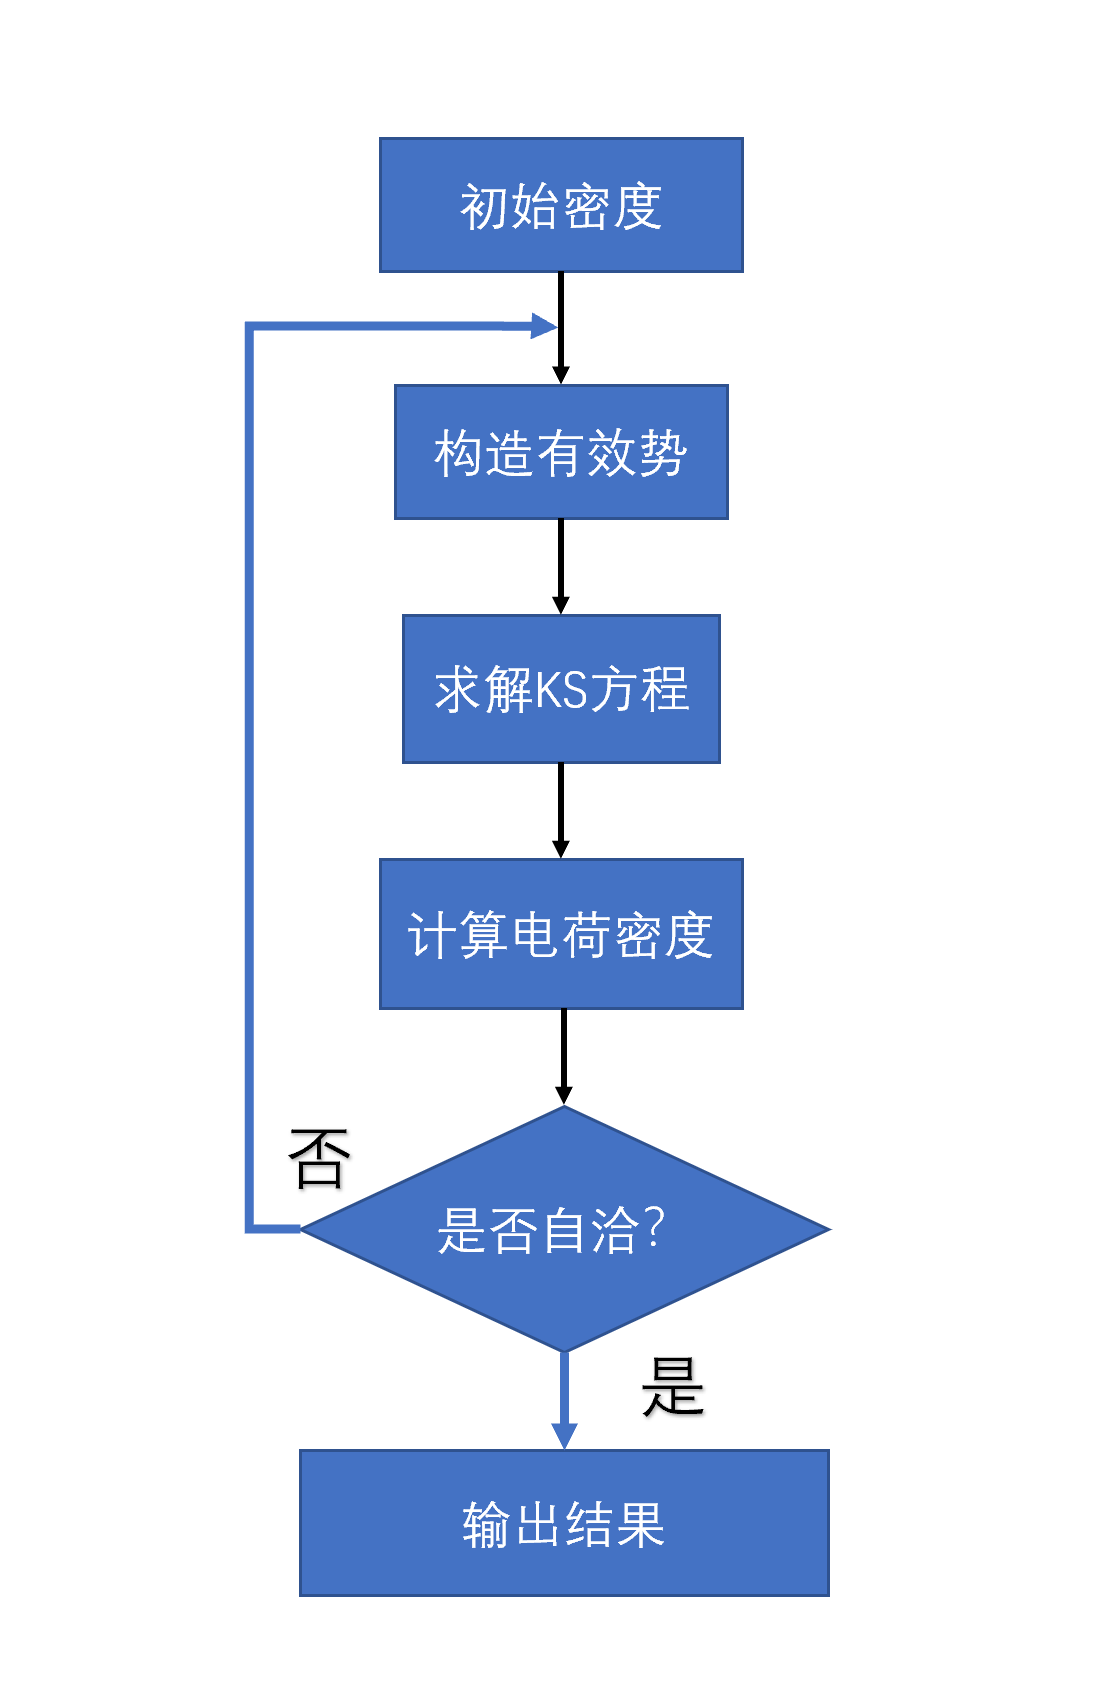
\includegraphics[width=0.5\textwidth]{./pic/012.png}
\caption{自洽求解KS方程流程图}

\label{dog012}
\end{figure}

霍恩伯格和科恩证明了两个重要的定理,即霍恩伯格-科恩第一定理与霍恩伯格-科恩第二定理,是密度泛函理论的基础。

\paragraph{霍恩伯格-科恩第一定理}
对于一个多粒子系统,外场$V(r)$是粒子密度分布函数$\rho(r)$的唯一泛函。由于外场确定后整个系统的哈密顿量就确定了,因此多粒子系统的基态也是密度分布函数的唯一泛函。

\paragraph{霍恩伯格-科恩第二定理}
如果是真实正确的电子密度分布函数,所得到的能量一定是最小值,即是所谓的变分原理。在实际使用时,如果采用近似的哈密顿量,得到的结果有可能会小于基态能量。

基于以上几个理论,可以得出与之对应的霍恩伯格-科恩泛函。
$$F_{HF}[\rho]=\min_{\Phi \to \rho} \langle {\Phi} |\hat{T}+\hat{U}_{ee}|\Phi \rangle =T[\rho]+U_{ee}[\rho]   $$

其中$T[\rho]$和$U_{ee}[\rho]$分别为电子动能泛函与库伦势能泛函。体系的总能量泛函可以写成:
$$E[\rho]=F_{HF}[\rho]+\int \rho(r)V(r)dr=T[\rho]+U_{ee}[\rho]+V[\rho]$$
由粒子总数为定值这一限定条件,求解体系能量最小值,可以应用拉格朗日乘数法等方式找到最低能量和与最低能量相一致的密度分布。在约束条件粒子总数为N,可以导出:
$$\delta\{T[\rho]+U_{ee}[\rho]+V[\rho] - \mu[\int \rho(r)V(r)dr-N]   \} =0$$
直接写出上面各项是十分困难的,需要进一步的近似处理。\cite{becke1992density}
对电子间相互作用这一项,可以写成两部分,一部分与库伦势能平方反比有关,另一部分是交换关联泛函,电子间的交换相关来源于费米子的反对称特性,是所有计算之中最复杂的一部分。
$$ U_{ee} = \frac{1}{2} \iint \frac{\rho (r) \rho (r') }{|r-r'|} drdr'+E_{XC}$$

Kohn和Sham提出过一个利用辅助的等价的无相互作用粒子系统的动能($T_{R}[\rho]$)替代由相互作用的系统的动能($T[\rho]$)。
$$F[\rho]=T_{R}[\rho]+\frac{1}{2} \iint \frac{\rho (r) \rho (r') }{|r-r'|} drdr'+E_{XC}$$
由薛定谔方程及动能算符可得
$$T_{R}[\rho]=\sum_{n = 1}^{N}\langle \Phi_{i} | -\frac{1}{2} \nabla^{2}| \Phi_{i} \rangle   $$
系统的能量泛函可以写成
$$E_{KS}[\rho]=\int \rho(r)V(r)dr+T_{R}[\rho]+\frac{1}{2} \iint \frac{\rho (r) \rho (r') }{|r-r'|} drdr'+E_{XC}$$
对总能量泛函做变分,最终可以得到著名的自洽KS方程\cite{kohn1965self}:
$$[-\frac{1}{2} \nabla^{2}+V_{eff}^{(i)}]\varphi_{i,s}(r)= \varepsilon _{i,s}\varphi_{i,s}(r)$$
$$V_{eff}=V(r)+\iint \frac{ \rho (r') }{|r-r'|} drdr'+\frac{\delta E_{XC}[\rho]}{\delta \rho[r]}$$
$$\rho(r)=\sum_{i = 1}^{N} \sum_{s = 1}^{2}|\varphi_{i,s}(r)|^{2}   $$
当交换关联能泛函形式确定之后,即可通过迭代方法求解KS方程。

对交换关联能的近似需要在满足关联函数对称性和求和规则,常用是近似方法有局域密度近似、广义梯度近似、meta-GGA泛函、杂化泛函等。
\paragraph{局域密度近似}局域密度近似(LDA)基本思想是将非均匀电子气看作是有无穷小体积元内部局域均匀电子气组成,利用均匀电子气的交换关联来近似非均匀电子气。经过近似之后可以得到交换关联泛函:
$$E_{XC}^{LDA}[\rho_{\uparrow}(r),\rho_{\downarrow}(r)]=\int [\rho_{\uparrow }(r)+\rho_{\downarrow}(r)]\varepsilon _{XC}^{h}[\rho_{\uparrow}(r),\rho_{\downarrow}(r)]dr$$
其中$\rho_{\uparrow}(r),\rho_{\downarrow}(r)$分别代表上自旋与下自旋的电子密度,$\varepsilon _{XC}$为均匀电子气的交换关联能密度。局域密度近似更适用于均匀密度体系,在非均匀密度体系,如原子体系,金属表面等与实际情况差异较大。\cite{黄美纯2000密度泛函理论的若干进展}
\paragraph{广义梯度近似} 广义梯度近似(GAA),是将交换关联能按照电子密度及其梯度展开:

$$E_{XC}[\rho]=\int \rho(r) \varepsilon _{XC} [\rho (r)]dr+\int F_{XC}[\rho (r) , \nabla   \rho(r)]dr $$

其中$\varepsilon_{XC}$为电子关联能密度,$F_{XC}$是与某些交换关联空穴性质有关的泛函。
\paragraph{meta-GGA泛函} meta-GGA泛函通过引入轨道动能密度,对广义梯度近似进行修正和改进。
$$E_{XC}^{meta-GGA}[\rho(r)]=\int \rho(r)\varepsilon_{XC}[\rho(r),\nabla \rho(r),\nabla^{2} \rho(r),\tau]dr$$
$$\tau(r)=\sum_{i} |\nabla\Phi_{i} | ^{2}$$
\paragraph{杂化泛函} 通过对GGA与HF形式的交换能按照一定比例混合起来,得到杂化泛函。类似的,可以同时把多种近似形式混合起来。不同的混合方式与混合比例所得到的杂化泛函有着不同的特点与作用形式。

求解KS方程固然可以使用变分法,但是最常用的是自洽场方法。\cite{黄时中1998双电子体系的简单自洽场计算} 自洽场方法首先猜测一个初始的电荷密度,通过这个电荷密度构造出有效势与哈密顿量。通过这个哈密顿量可以解得波函数与能量本征值。所得的波函数又可以重新构造一个电荷密度。利用新得到的电荷密度代替原来的电荷密度,然后反复迭代循环。如果前后两次得到的电荷密度相差达到所设定的精度差,即可认为电荷密度已经收敛。

\section{对称性与空间群}

在凝聚态物理的研究中,对称性有着极其重要的地位,物质的各种存在形式都有着或多或少的对称性,对物质性质变化其决定性作用的相变也与对称性的产生与消失有着密切的联系。在多铁二维材料的研究中,铁磁性与铁电性的出现基本上都是与一种或多种的对称性破缺有关,在高对称结构中寻找对称性的破缺是寻找铁电铁磁材料的关键点之一。

\subsection{对称性极其操作}

对于某些物理量$\rho(r)$,以与空间位置r有关,可以引入一个坐标变换的操作g,使得坐标按照一定的规则发生变化:
\begin{equation}
    \bm{r} \rightarrow  g\bm{r} = \bm{r}'
\end{equation}
坐标的变化同样会使得依赖于坐标的物理量发生变化,如果这个物理量在变化前后依然相等,那么这个物理量在变换操作g下具有对称性。
\begin{equation}
    \rho (\bm{r}') = \rho (g \bm{r}) = \rho (\bm{r})
\end{equation}

在三维空间中,可以简单地采用直角坐标系来表示一个点的位置,而对坐标的变化操作可以分解为两部分,平移部分与非平移部分。平移部分可以用位矢的直接相加减来描述,非平移部分可以采用矩阵乘法来描述:
\begin{gather}
    \bm{r}(x,y,z) \rightarrow \bm{r}'(x',y',z') \\
    \bm{r}'=g\bm{r}=\bm{M}\bm{r}+\bm{t} \\
    \bm{M}=(a_{ij})= \begin{pmatrix}
        a_{11}&a_{12}&a_{13}\\
        a_{21}&a_{22}&a_{23}\\
        a_{31}&a_{32}&a_{33}
    \end{pmatrix}
    \\
    x_{i}' = \sum_{j} a_{ij} x_{j}+t_{i}
\end{gather}
对于狭义的对称性来说,对象内部任意两点的直线距离不会发生变化,这意味着在狭义对称操作下,被操作对象不会发生膨胀与压缩现象。

对与点对称,变换矩阵的行列式应该满足矩阵的行列式的绝对值为1,即:
\begin{equation}
    |\bm{M}|=|a_{ij}|=\pm 1
\end{equation}
以绕Z轴从α转动到β为例:
\begin{equation}
    \bm{M}_{1} = 
    \begin{pmatrix}
        cos(\beta - \alpha) & -sin(\beta - \alpha) & 0\\
        sin(\beta - \alpha) & cos(\beta - \alpha) & 0\\
        0 & 0 & 1 
    \end{pmatrix}
\end{equation}
对与以XY平面为对称面的面对称操作:
\begin{equation}
    \bm{M}_{2} = \begin{pmatrix}
        1 & 0&0\\
        0&1&0\\
        0&0&-1
    \end{pmatrix}
\end{equation}
对坐标原点的中心反演对称操作:
\begin{equation}
    \bm{M}_{3} = \begin{pmatrix}
        -1 & 0&0\\
        0&-1&0\\
        0&0&-1
    \end{pmatrix}
\end{equation}
通过观察计算$M_{1}M_{2}M_{3}$可以发现,$|M_{1}|=+1$而$M_{2}M_{3}$的绝对值为-1。通过对变化矩阵行列式的计算,可以将变化g分为两类$g^{\uppercase\expandafter{\romannumeral1}}g^{\uppercase\expandafter{\romannumeral2}}$,一种变换矩阵的行列式为正,另一种变换矩阵的行列式为负。对与多次连续变换,依据矩阵乘法与行列式规则可以得到,第一类变换的组合或连续变换的结果仍然为第一类变换,第二类变换的偶数次连续变换为第一类变换,奇数次变换为第二类变换:
\begin{equation}
    |\bm{M}(g)|= | \bm{M}(g_{1}^{\uppercase\expandafter{\romannumeral2}}  g_{2}^{\uppercase\expandafter{\romannumeral2}} g_{3}^{\text{\uppercase\expandafter{\romannumeral2}}} \cdots g_{q}^{\uppercase\expandafter{\romannumeral2}})|=(-1)^{q}= \begin{cases}
        +1, &\text{q为偶数}\\
        -1, &\text{q为奇数}
    \end{cases}
\end{equation}

除了行列式上的不同之外,这两类变换还有着更明显更加显著的区别,第一种变换可以通过物体在空间位置上的运动来实现,而第二种对称变换操作则不能在实空间内通过位置的改变实现,必须同过别的方式变换,以手性分子为例,左旋分子是无法在不改变化学键的基础上仅仅通过空间运动来转化成为右旋分子的。

\begin{figure}[]
    \centering
    \resizebox{\textwidth}{!}{
        \subfigure[]{
            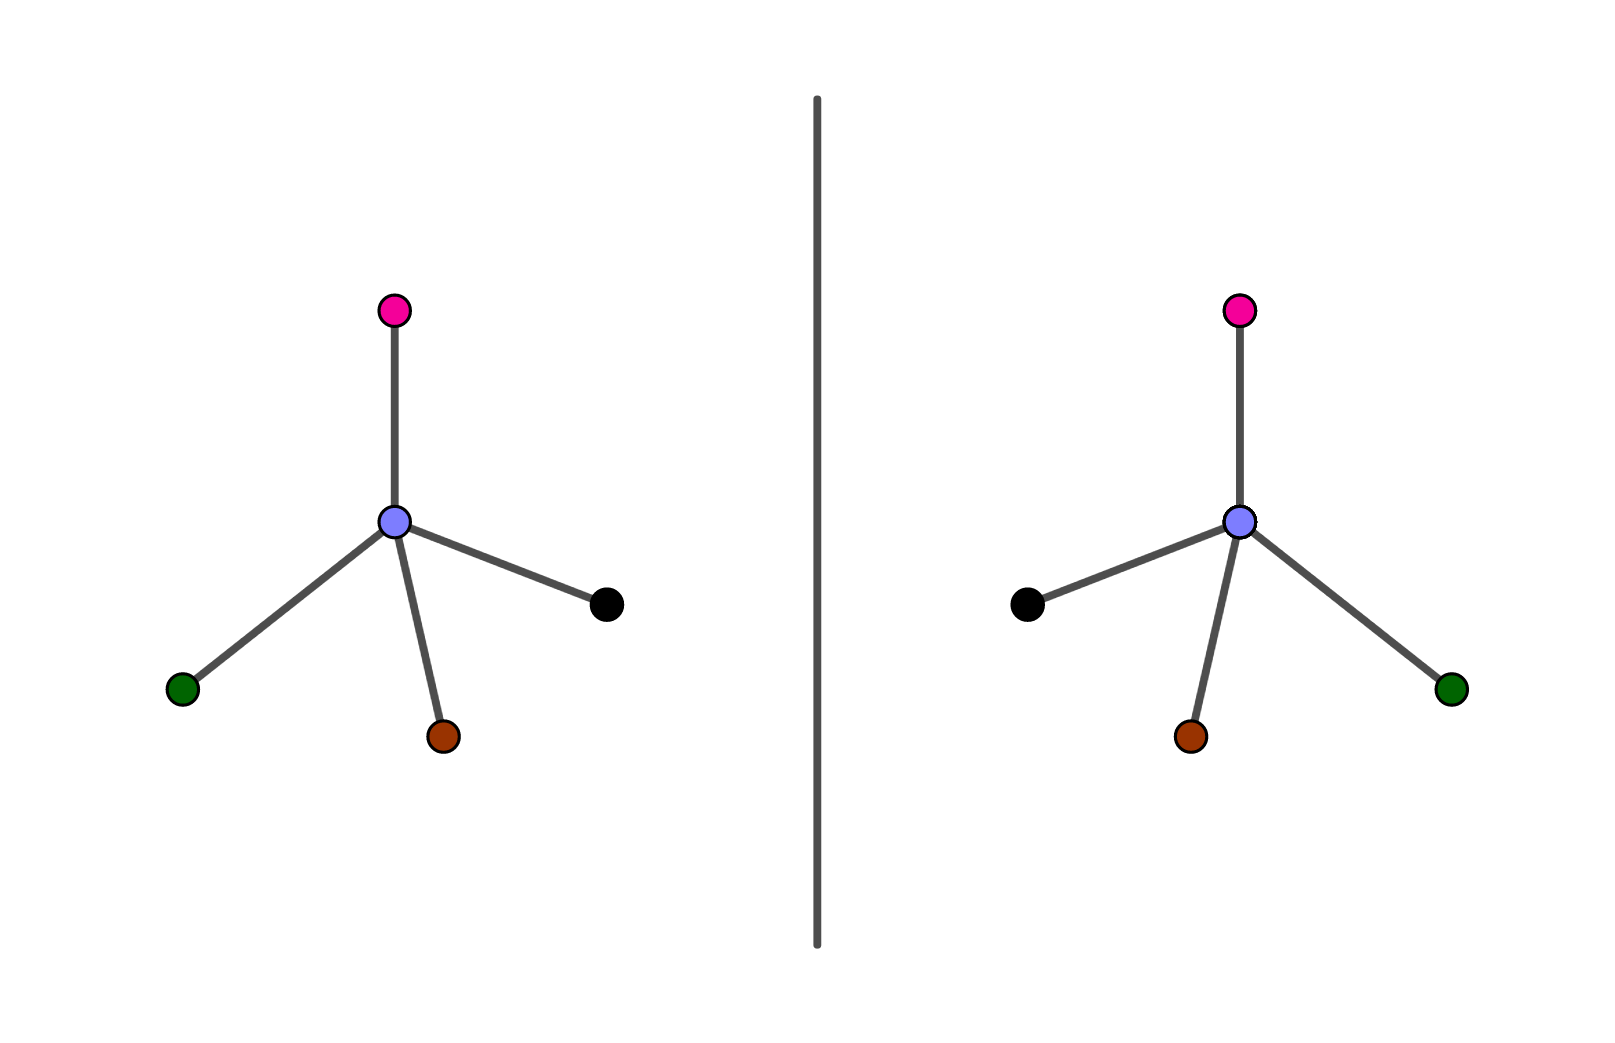
\includegraphics[]{pic/p007.png}
        }
        \subfigure[]{
            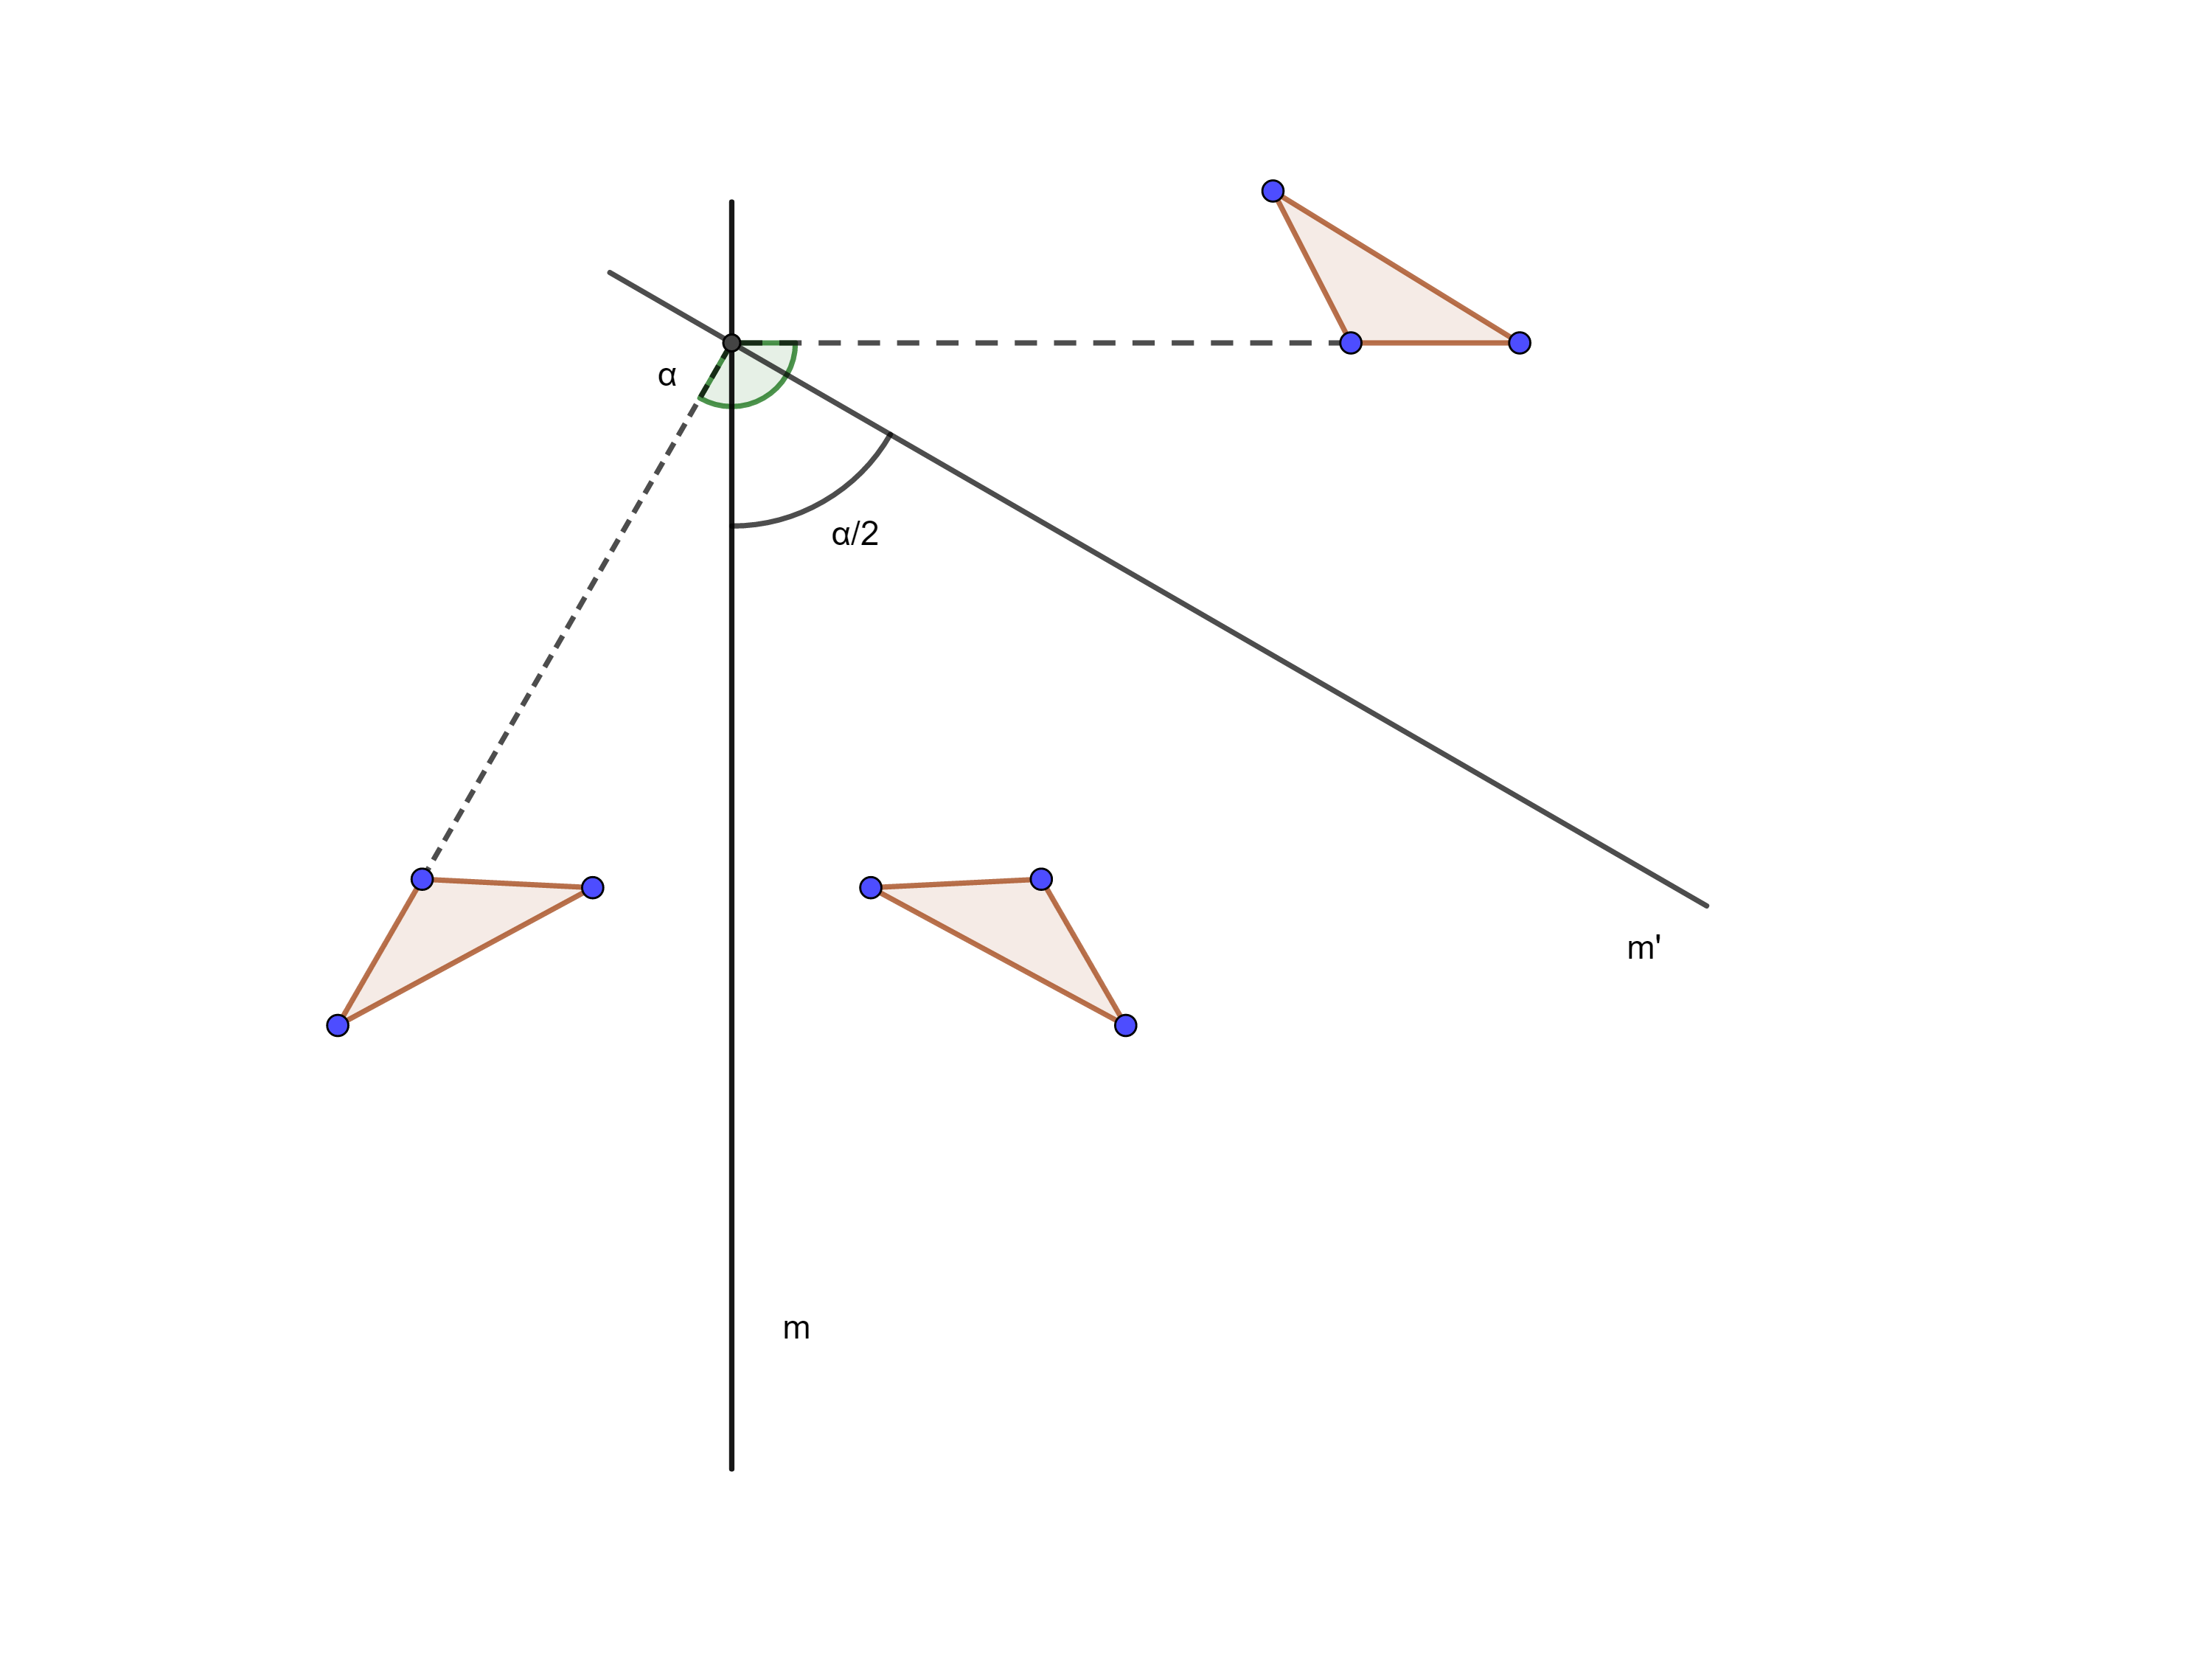
\includegraphics[]{pic/p006.png}
        }
    }
    \caption{(a)手性分子的对称性,左旋分子无法通过空间位置操作转化为右旋分子。(b)万花筒定理}
    \label{p006p007}
\end{figure}

\subsection{对称元素的组合定理}

\paragraph{镜面旋转与反演旋转等价}
镜面旋转$\tilde{N}_{\alpha} $与反演旋转$\bar{N}_{\beta}$等价,即$\tilde{N}_{\alpha} =  \bar{N}_{\pi - \alpha}$。

\paragraph{万花筒定理}
当两个夹角为$\alpha/2$的镜面m与m'的交线相当于转轴$N_{\alpha}$,这个定理是用来制作万花筒的理论依据。

\paragraph{Euler定理}
绕两条相交转轴$N_{\alpha 1}\text{和}N_{\alpha 2}$的先后两次旋转相当于绕第三条轴$N_{\alpha 3}$的旋转,即:
\begin{equation}
    N_{\alpha 1} +N_{\alpha 2}=N_{\alpha 3}
\end{equation}

这三条定理大大减少了对称性元素的组合复杂度,使得对称性理论变得简单。

\subsection{对称群}

对称性与对称性的组合问题需要用群论这个数学工具才能更好地研究明白,一个确定物体的所有对称性操作构成一个对称群的一组元素。群是群论的核心内容,群的概念由群的四个公理定义出来:

\paragraph{封闭性}
群元素的乘积也是一个群元素,以对称群为例,对称群中的两个元素的乘积,也就是两种对称性操作的连续操作等效与群中的另外一个元素(操作),即:$g_{i} \in G , g_{j} \in G  \rightarrow g_{i}g_{j} =g_{l} \in G $。

\paragraph{结合律}
群元素的乘积满足结合律,即:$g_{i}(g_{j}g_{l})=(g_{i}g_{j})g_{l}$。

\paragraph{存在恒等元素}
存在恒等元素e,使得$\text{对于任何}g_{i} \in G \text{,都有} eg_{i}=g_{i}$。

\paragraph{存在逆元素}
对于G中任一元素$g_{i}\text{都有一个逆元素}g^{-1}_{i}\text{使得}g_{i}g_{i}^{-1}=e$。

在通常的群中,一般不存在交换律或交换律不成立,即$g_{i}g_{j} \neq g_{j}g_{i}$,群元素交换次序之后和原来不同,但在特殊的阿贝尔群中,两个元素交换不变$g_{i}g_{j} = g_{j}g_{i}$。不同的群有着不同数目的元素,一个群中包含的元素数目叫群的阶。在一个群内部,如果挑选出部分元素,仍然符合群的定义,可以组成一个规模比较小的子群,子群的阶数一般会小于原来群的阶数。

\subsection{二维平面周期性结构}

周期性原子排列不仅仅是普通的三维材料的研究重点,在二维材料中也是一个十分重要的方面。在三维空间中有着十四种布喇菲格子,但在二维空间中由于对称性比三维空间中要更简单,二维空间中仅有五种布喇菲格子,分别为:斜方、长方、菱形、正方和六角。


\begin{figure}[htbp]
    \centering
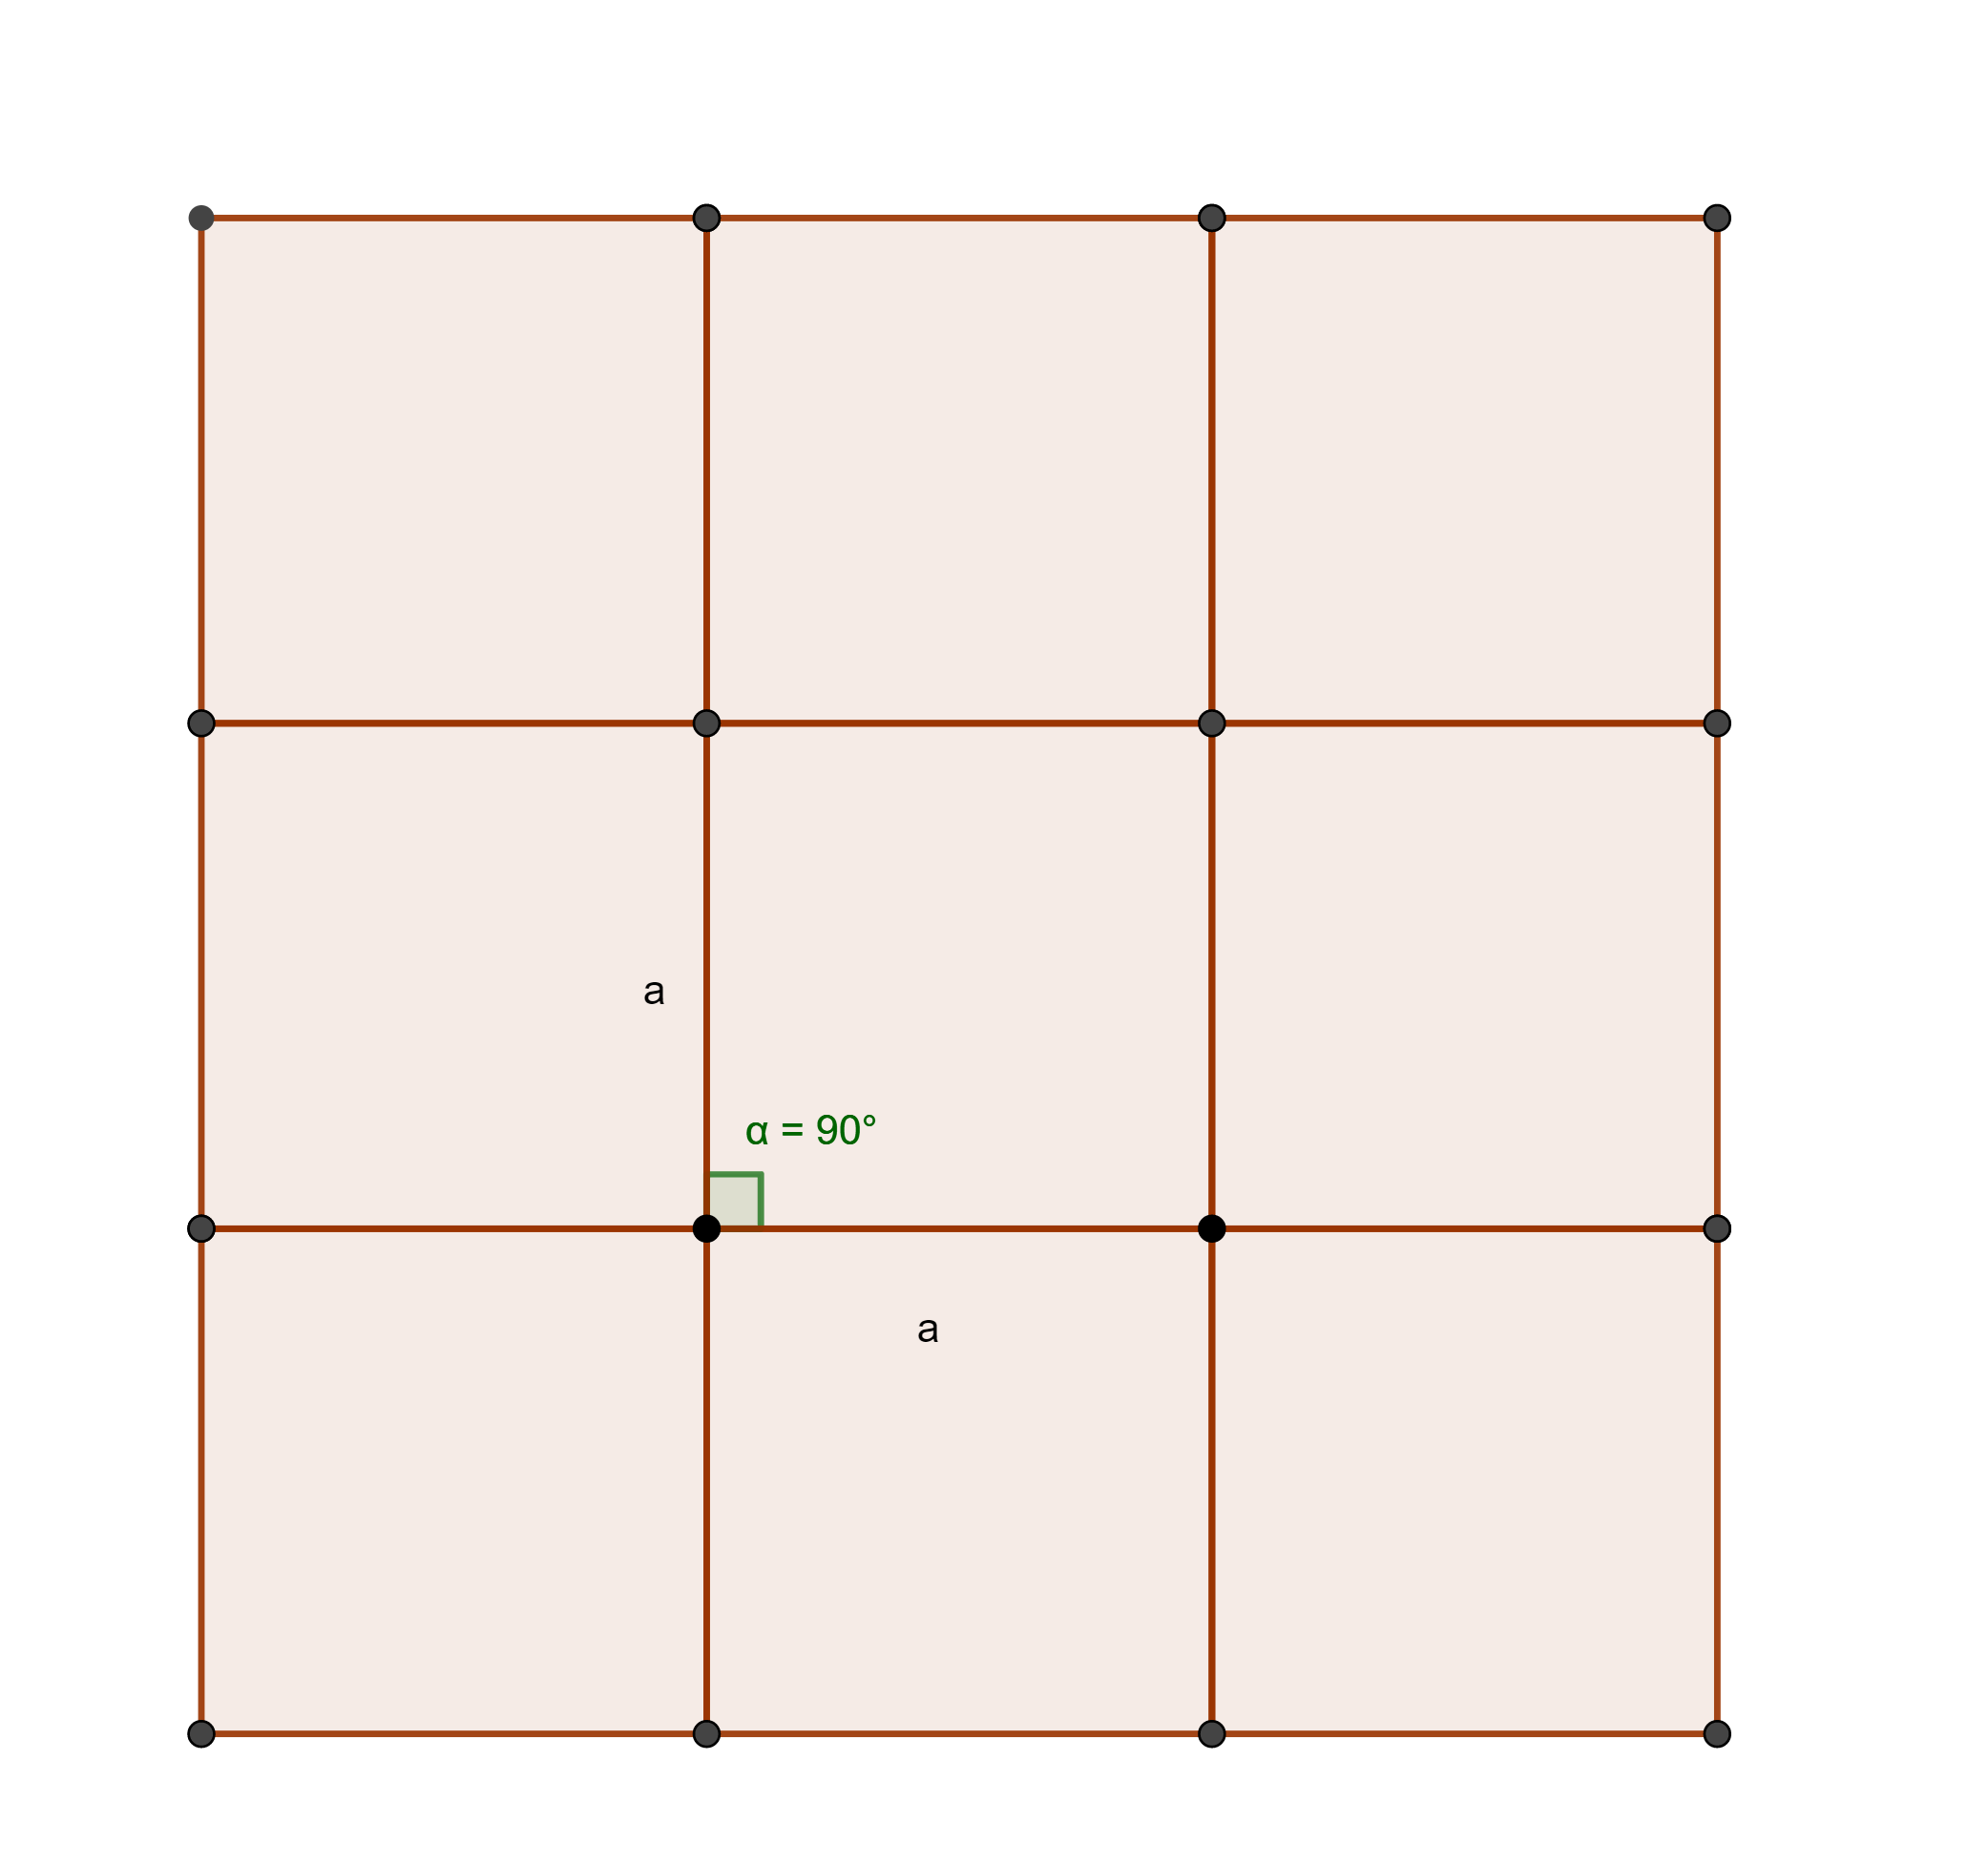
\includegraphics[width=0.4\textwidth]{./pic/p008-1.png}
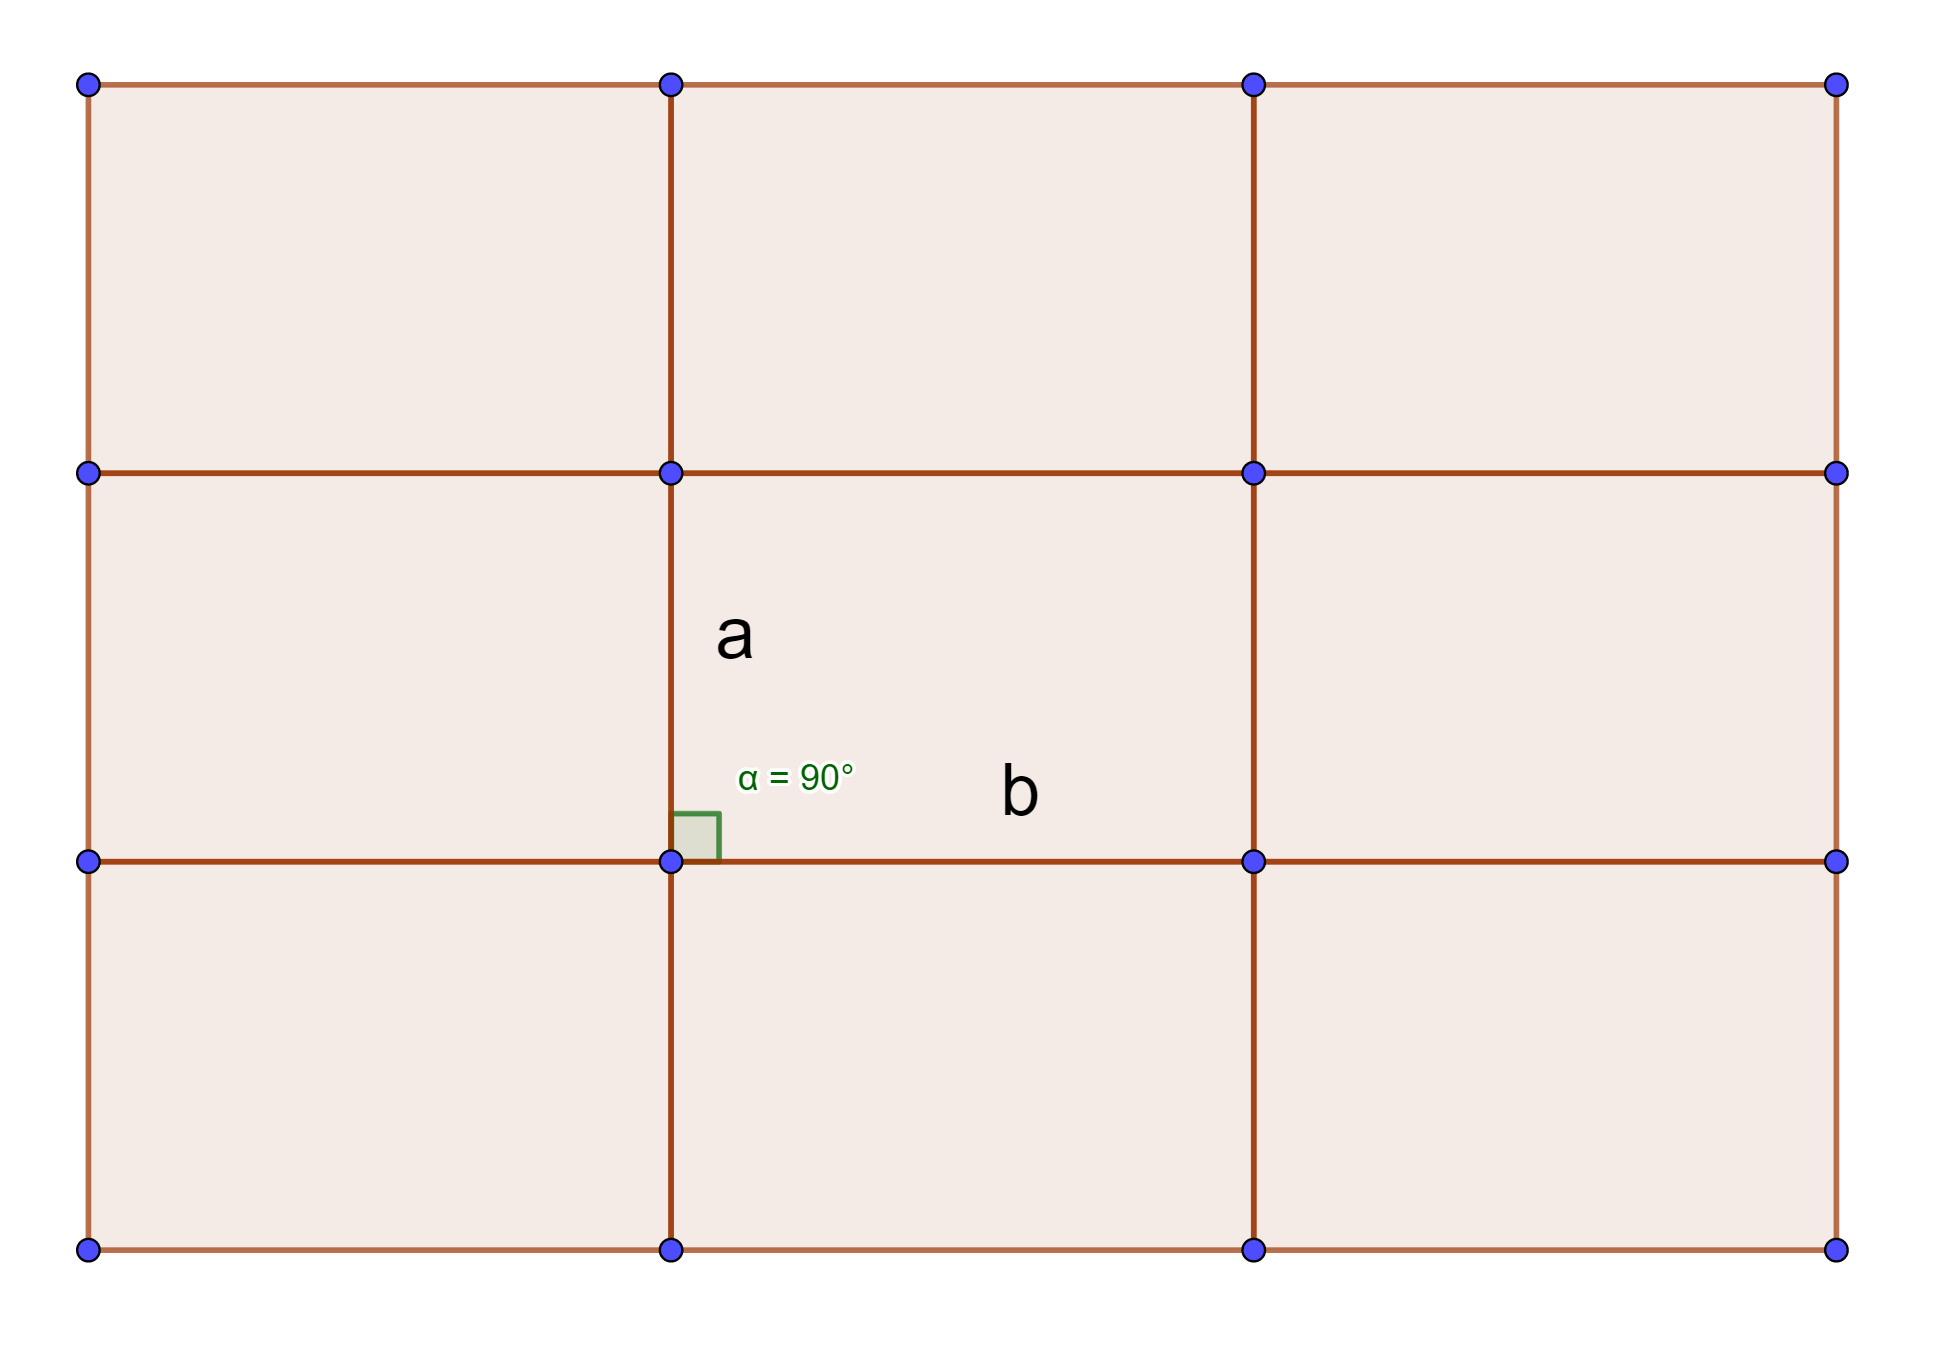
\includegraphics[width=0.4\textwidth]{./pic/p008-2.png}
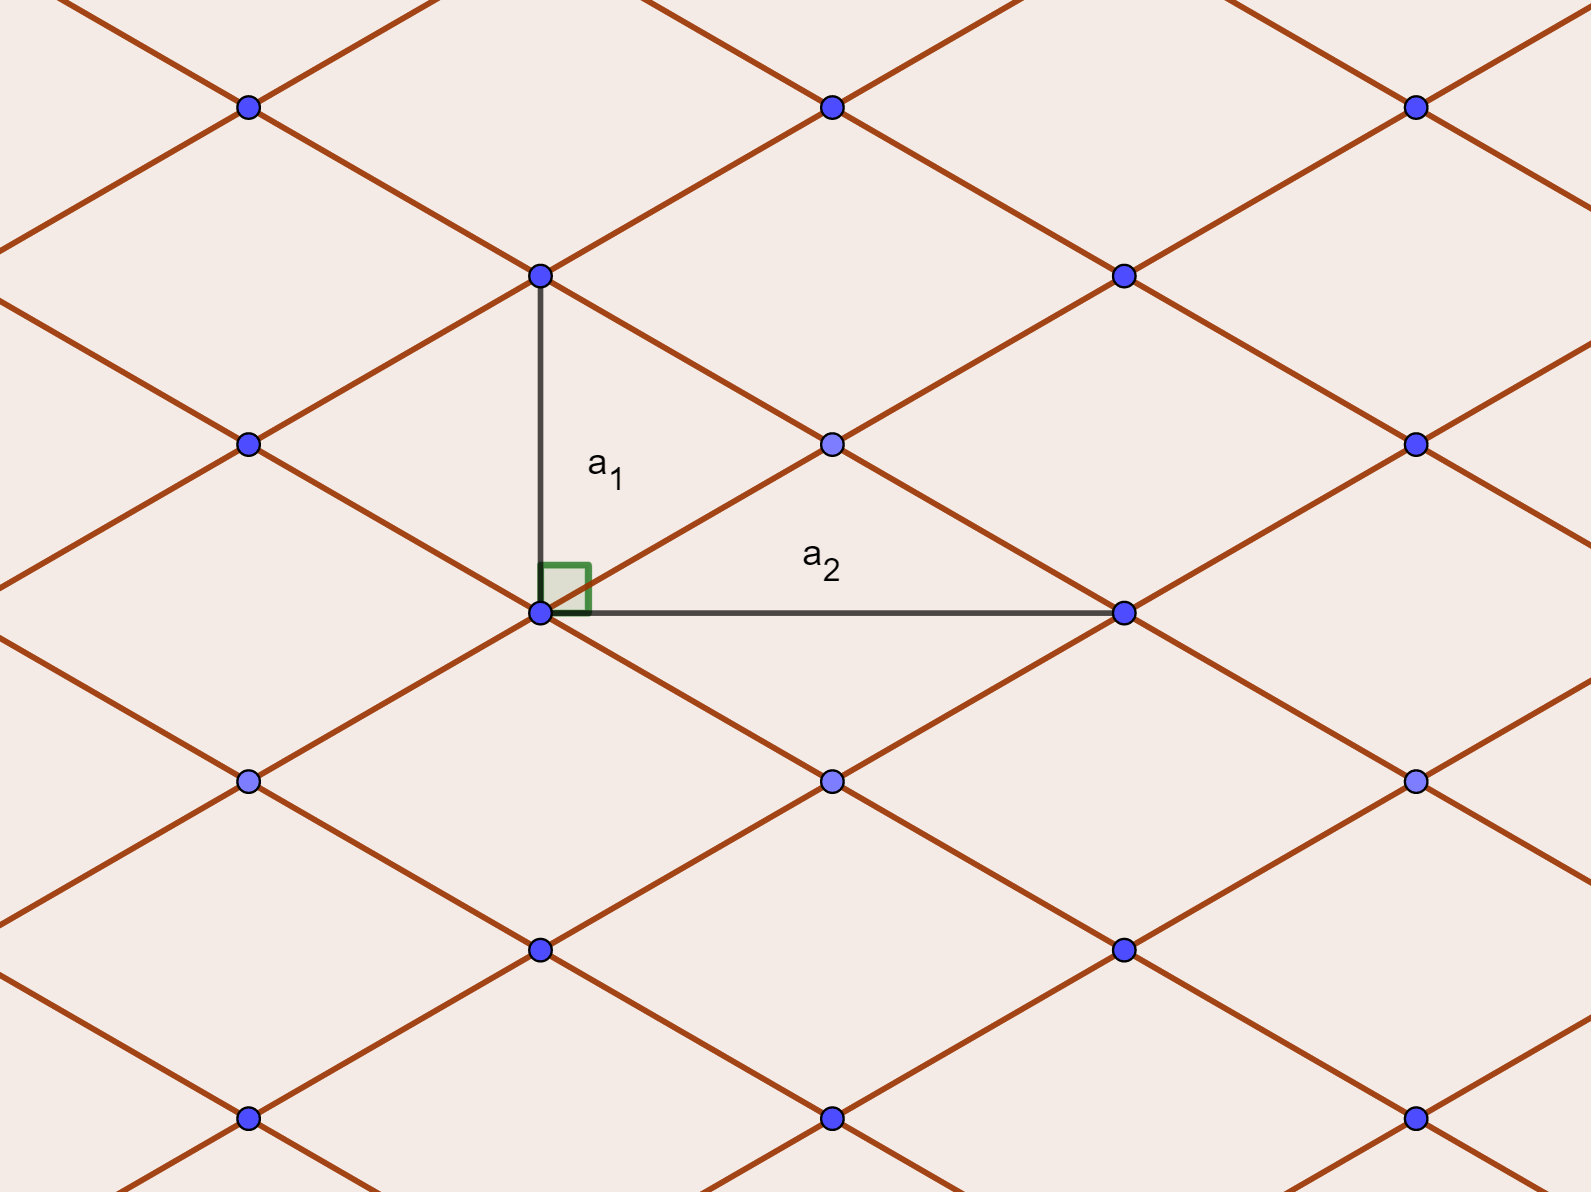
\includegraphics[width=0.3\textwidth]{./pic/p008-3.png}
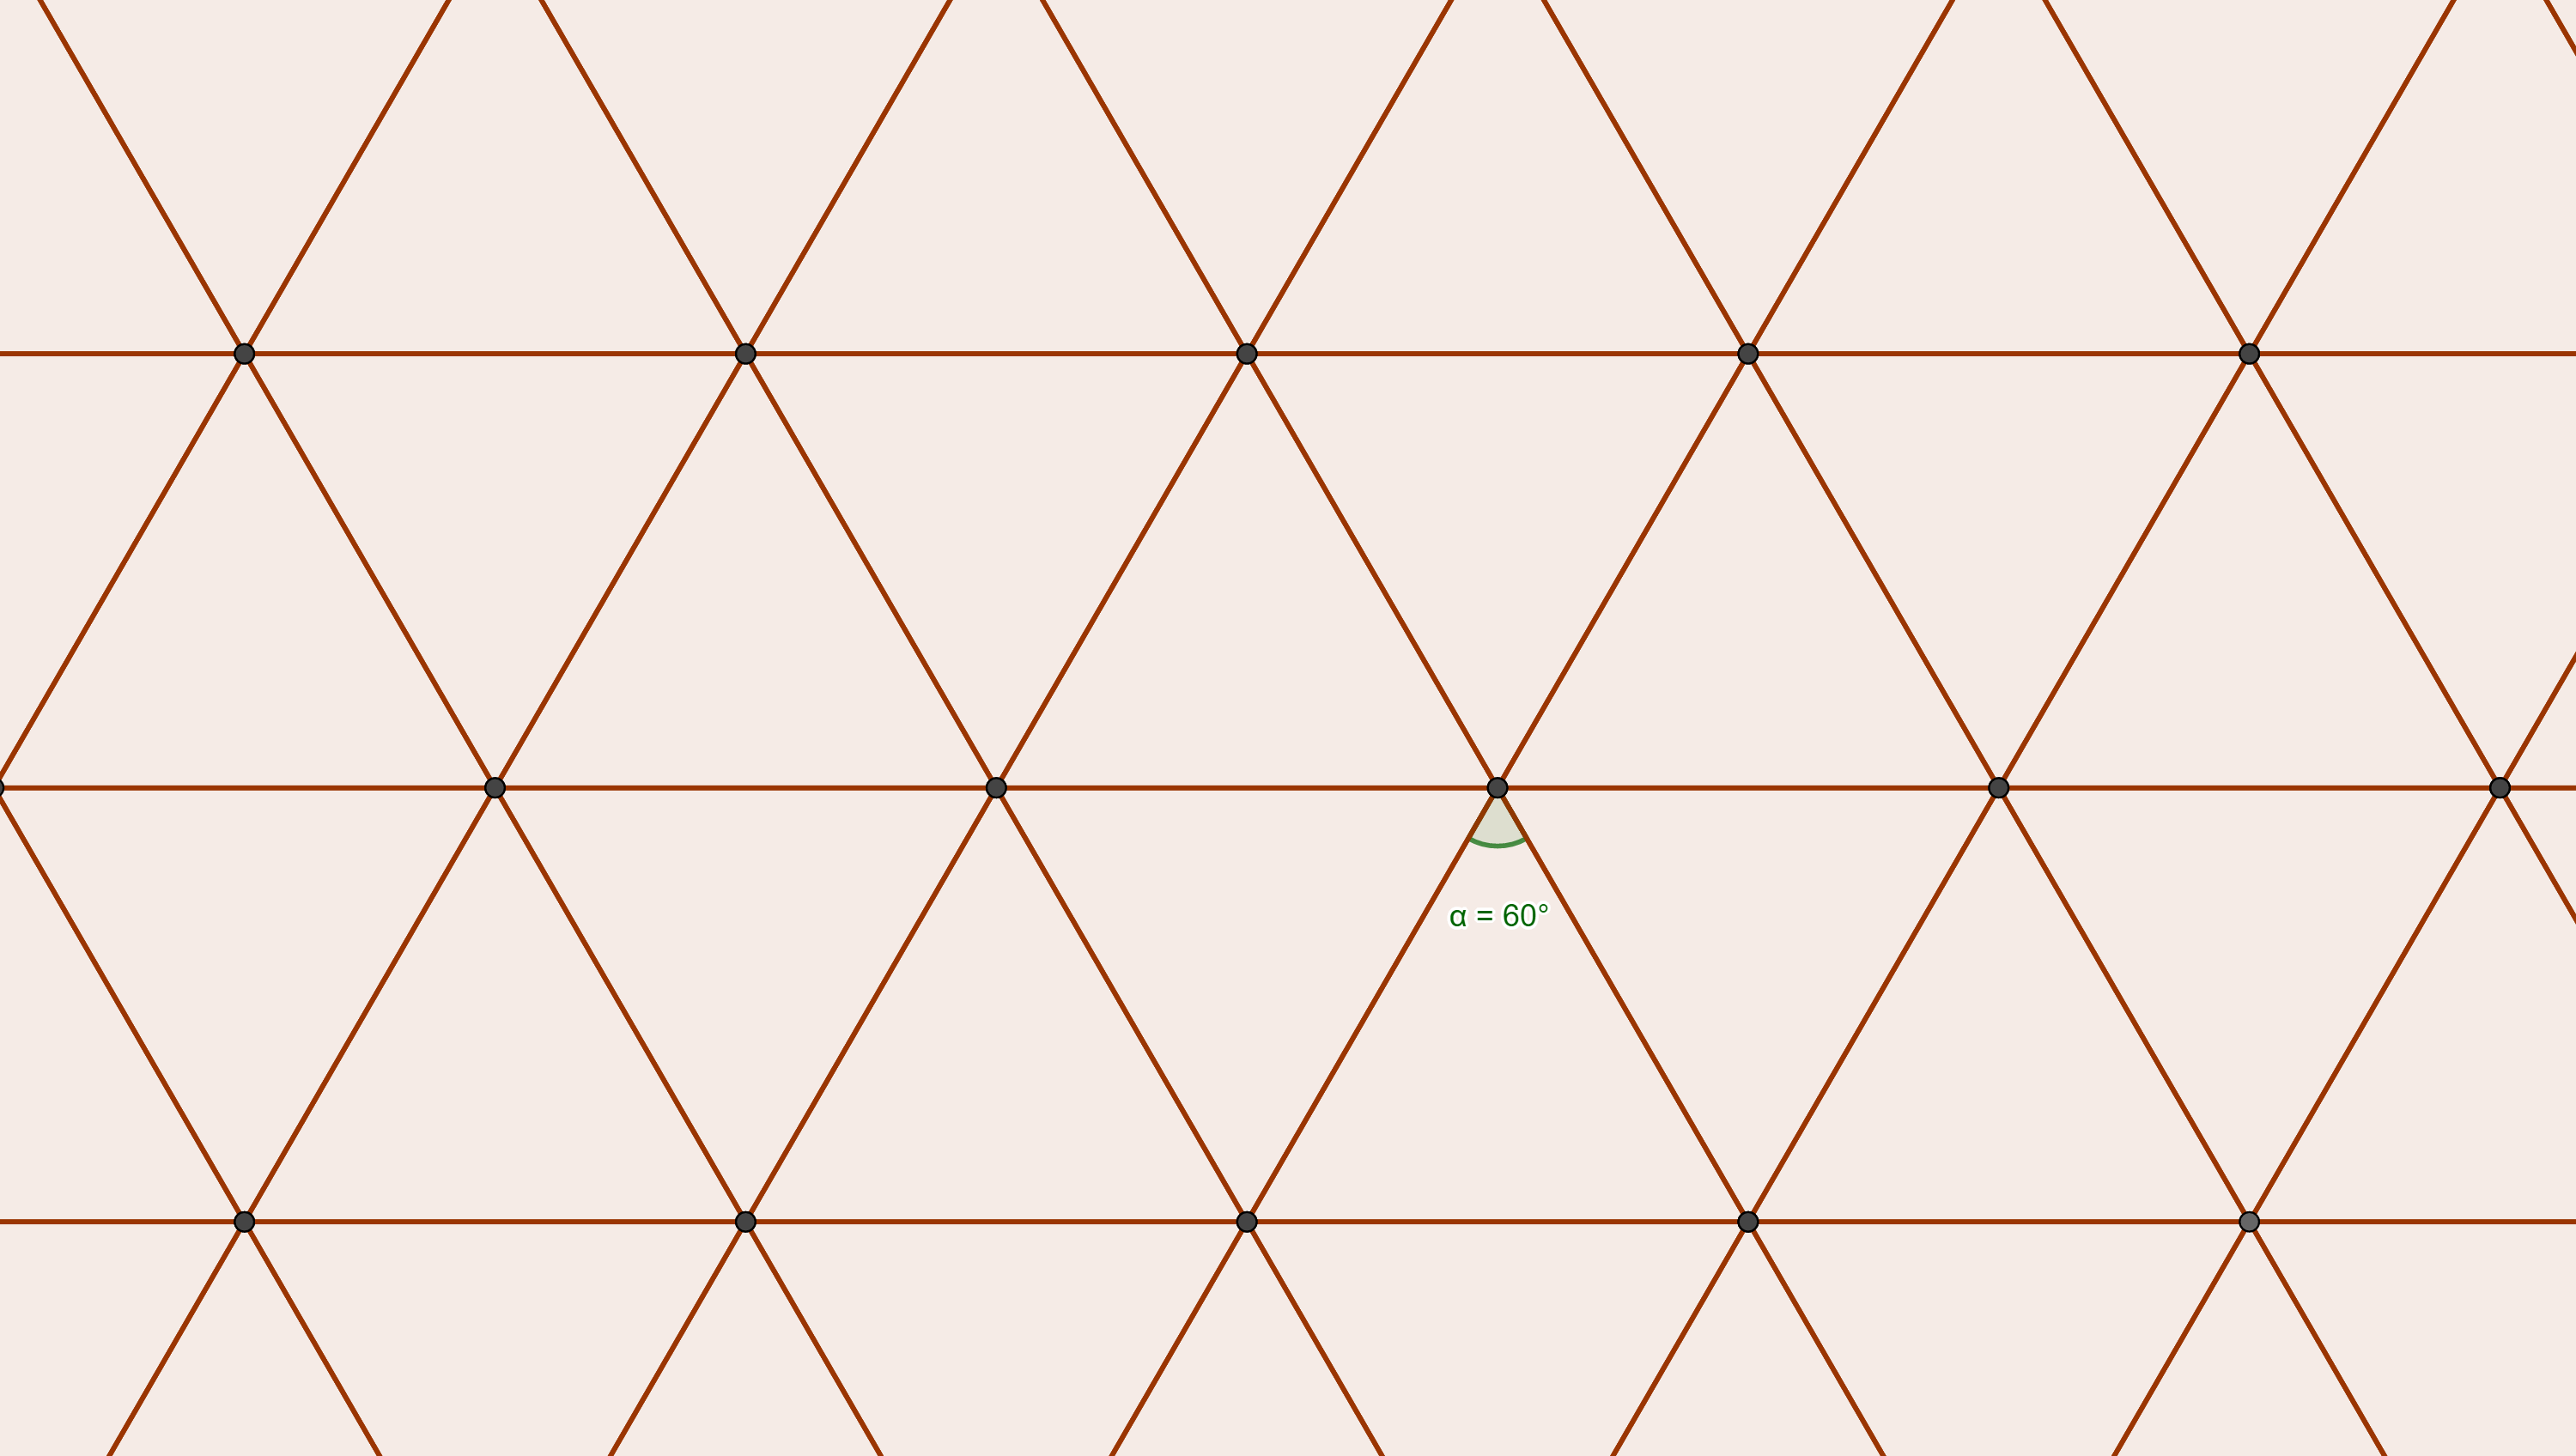
\includegraphics[width=0.3\textwidth]{./pic/p008-4.png}
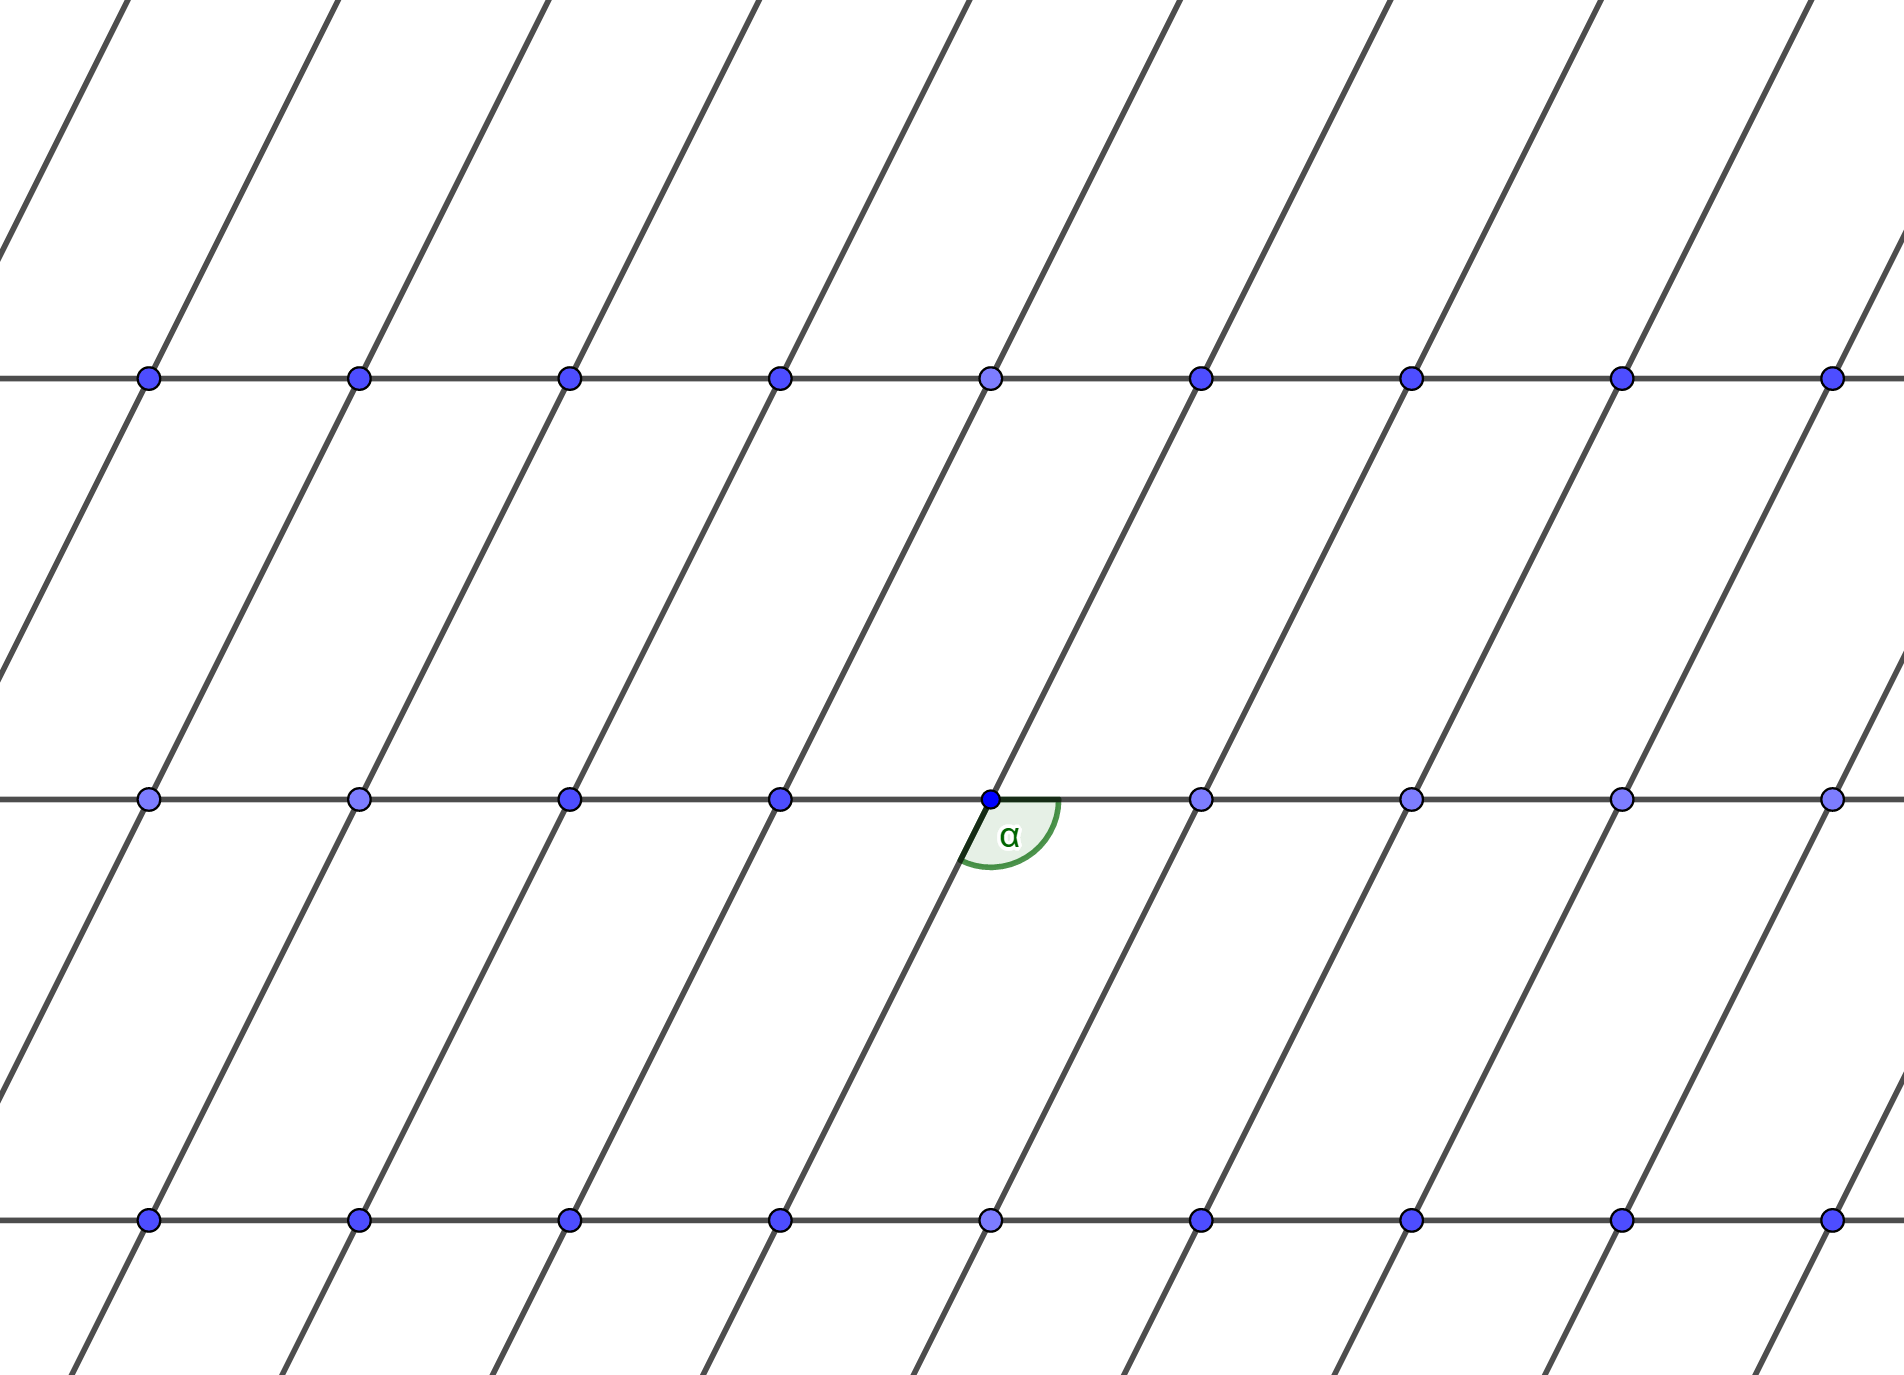
\includegraphics[width=0.3\textwidth]{./pic/p008-5.png}

\caption{二维空间中的五种布喇菲格子}

\label{dogp08}
\end{figure}
% \end{document}





